% \documentclass[11pt]{article}
%\documentclass[review]{elsarticle}
\documentclass[5p,times]{elsarticle}
\usepackage{lineno,hyperref}
% \modulolinenumbers[5]
% \linenumbers
% \journal{Egyptian Informatics Journal}
% -----------------------------
% Packages (minimal, common)
% -----------------------------
% \usepackage[a4paper,margin=1in]{geometry}
\usepackage{microtype}
\usepackage{hyperref}
\usepackage{enumitem}
\usepackage{graphicx}
\usepackage{booktabs}
\usepackage{amsmath,amssymb}
\usepackage{tikz}
\usetikzlibrary{shapes.geometric, shapes.symbols, arrows.meta, positioning, fit, backgrounds, calc}
\usepackage{float}
\usepackage{todonotes}
\usepackage{tabularx}
\usepackage{multirow}
\usepackage{seqsplit}
\newcommand{\schema}[1]{\texttt{\seqsplit{#1}}}
% -----------------------------
% Metadata
% -----------------------------

% \author{, Ahmed Awad}
% \date{\today}
\journal{Future Generation Computer Systems}
\begin{document}
\begin{frontmatter}
    % \title{STREAMTRACK: Multi-Camera Object Tracking Using Streams and Tables}
    \title{STREAMTRACK: A Streams-and-Tables Architecture for Scalable and Reconfigurable Multi-Camera Object Tracking}
%      \author[add3,add2]{Ahmed Awad\corref{mycorrespondingauthor}\fnref{equal}}
%     \cortext[mycorrespondingauthor]{Corresponding author}
%     \ead{ahmed.awad@buid.ac.ae}
    
%     \author[add1]{Mahmoud Tayee\fnref{equal}}%\email{23001546@ug.buid.ac.ae}
%     \ead{m.mostafa2118@nu.edu.eg}
  

%     \author[add1]{Mohamed ElHelw}
%     \ead{melhelw@nu.edu.eg}
% \address[add3]{The British University in Dubai, Dubai, The UAE}
% \address[add1]{Nile University, Giza, Egypt}
% \address[add2]{Faculty of Computers and Artificial Intelligence, Cairo University, Egypt}
% \fntext[equal]{These authors contributed equally to this work.}

\begin{abstract}
Multi-camera object tracking (MCOT) is typically built as a tightly coupled, monolithic computer-vision pipeline, which makes cross-camera association hard to scale, identity decisions hard to inspect, and the camera network hard to reconfigure. We argue these are problems of \emph{architecture}, not of the vision task, and re-architect MCOT as a \emph{streams-and-tables} system: detections flow as streams, global identities and camera topology are queryable relational tables, and cross-camera association is a continuous, topology-aware join over them. 
This turns each difficulty into a property of the design: topology-pruned association (scalability), an inspectable identity view (observability), and topology-as-data (zero-downtime reconfigurability). Realised on an embeddable complex-event-processing engine, the architecture reproduces the
global-identity assignments of a state-of-the-art batch baseline while delivering a \textbf{9.8$\times$} overall speedup (up to \textbf{12.0$\times$} in representative selection and \textbf{9.5$\times$} in clustering) over an equivalent JVM-native batch implementation, isolating the architectural speedup from language, runtime, and library effects, with a further \textbf{4.16$\times$} latency reduction (\textbf{4.27$\times$} in
 steady state) from topology-aware partitioning at nine cameras. 
 
 %The source code and instructions to reproduce the experiments are available at \url{https://github.com/MahmoudMostafaTayee/STREAMTRACK}.

\end{abstract}


\begin{keyword}
Stream Processing\sep Complex Event Processing\sep Software Architecture\sep Multi-camera Object Tracking\sep Streams and Tables\sep Edge Computing
\end{keyword}

\end{frontmatter}
% \maketitle


\section{Introduction}
\label{sec:intro}

Multi-camera object tracking (MCOT) underpins a growing class of applications, such as urban traffic management~\cite{9151096} and public-space surveillance~\cite{thirde2006multi,bhuyan2007tracking}.
%\todo{student[Done]: cite 2--3 representative MCOT application papers}. 
The task is to assign a single,
consistent global identity to each physical object as it moves across a network of cameras. Such systems must meet not only computer-vision accuracy targets but also operational
demands, scaling to more cameras, exposing intermediate decisions for debugging, and adapting to changes in the camera network topology.

These operational demands are where conventional MCOT systems struggle. We argue the cause is \emph{architectural} rather than algorithmic. Such systems are typically built as tightly coupled,
monolithic computer-vision pipelines in which cross-camera association logic, identity state, and
network topology are entangled in bespoke imperative code~\cite{yoshida2024overlap,kim2024cluster,xie2024robust}. %\todo{student[Done]: cite representative monolithic/MTMC pipelines, e.g. AI City Challenge entries}

This coupling is precisely what makes association hard to scale (matching defaults to all camera pairs), state hard to inspect (identity decisions live in in-memory program variables), and camera network topology hard to change (re-linking cameras means editing code and restarting the pipeline, losing accumulated state). Treating these as vision problems misdiagnoses them; they are consequences of the system's architecture.

We address them by re-architecting MCOT as a \emph{streams-and-tables} system, which we call \textbf{STREAMTRACK}. Per-camera detections and tracklet updates flow as append-only \emph{streams}; global identities and the
camera-network topology are maintained as mutable, queryable relational \emph{tables}; and cross-camera association is expressed as continuous CQL queries over them, realised as
topology-aware stream joins parametrised by a live camera-neighbourhood table. This rests on the
stream--table duality from data-stream management~\cite{sax2018streams,DBLP:conf/dbpl/ArasuBW03},
and is not specific to vision: the same paradigm has been shown to transform a stream engine into a process-orchestration engine~\cite{awad2025best}. Demonstrating it here on a problem as different as multi-camera perception is evidence that streams-and-tables is a general architectural approach for re-engineering monolithic, stateful reactive systems pipelines, not a one-off technique.

The reframing is valuable because it turns each operational difficulty into a property obtained by construction. Pruning association to topological neighbourhoods makes it \emph{scalable}; maintaining identity in a relational table makes the system's state \emph{inspectable}; and representing topology
as data makes the network \emph{reconfigurable at runtime}, \emph{without any code changes or pipeline restarts}.
We realise the architecture on Esper, an embeddable complex-event-processing engine, in a single process where high-dimensional appearance tensors are referenced by object identity and shared
in memory without serialisation.

This paper makes the following contributions:
\begin{itemize}[leftmargin=*]
    \item \textbf{A streams-and-tables re-architecting of MCOT.} We recast a representative monolithic multi-camera tracking pipeline as an operator graph over detection streams and
    relational state tables (global identities, camera topology), with cross-camera association expressed as continuous queries.
    \item \textbf{Topology-aware association as stream joins.} Cross-camera matching is a parametrised join over a live neighbourhood table, pruning all-pairs comparisons to localised ones and yielding a \textbf{4.16$\times$} per-association latency reduction (up to \textbf{4.27$\times$} in steady state excluding JVM warm-up) at nine cameras.
    \item \textbf{Topology as reconfigurable data.} Overlapping and transitional camera links are held in a single relational table, enabling zero-downtime reconfiguration of the network
    without code changes or loss of tracking state.
    \item \textbf{Deterministic, inspectable state management.} Global identity is a continuously materialised, queryable view, with priority-ordered timer queries bounding memory under sustained load.
    \item \textbf{An end-to-end realisation and evaluation on Esper.} The architecture reproduces the global-identity assignments of a state-of-the-art batch baseline
    (functional parity verified stage-by-stage on the Woven WTS dataset) while delivering a \textbf{9.8$\times$} overall speedup (clustering: \textbf{9.5$\times$};
    representative selection: \textbf{12.0$\times$}) over an equivalent JVM batch baseline, isolating the architectural speedup from language, runtime, and library
    effects\footnote{The original state-of-the-art pipeline is written in Python. We ported it to Java and validated the port against the original outputs to enable a fair, 
    same-runtime comparison.}; topology-aware partitioning and runtime reconfiguration are evaluated on the nine-camera NVIDIA SmartSpaces network, yielding a further
    \textbf{4.16$\times$} per-association latency reduction.
\end{itemize}
\looseness=-1
The remainder of the paper is organised as follows. Section~\ref{sec:background} defines the
problem and the streams-and-tables background. Section~\ref{sec:related} positions our work
against multi-camera tracking systems and stream-processing foundations, establishing the gap
we address. Section~\ref{sec:overview} presents the architecture, its operator model, and its
realisation on Esper. Sections~\ref{sec:single} and~\ref{sec:multi} detail the single-camera
and cross-camera operators together with their EPL realisations.
Section~\ref{sec:evaluation} reports the evaluation, and Section~\ref{sec:conclusion} concludes
with operational benefits, limitations, and future directions.

\section{Background and Problem Definition}\label{sec:background}

\subsection{Multi-Camera Object Tracking (MCOT)}
\label{sec:background:mcot}

We consider a set of cameras $\mathcal{C} = \{c_1,\dots,c_m\}$. Each camera $c$ produces a stream of detections $\mathcal{D}_c$, where each detection $d \in \mathcal{D}_c$ consists of a bounding box, an appearance embedding vector $f \in \mathbb{R}^{d}$, and a timestamp $t$. The goal of MCOT is to assign a \emph{global identity} $ID_G$ to each observation such that all detections of the same physical object across the camera network $\mathcal{C}$ share the same identity over time, producing consistent and continuous identity tracks.

This goal decomposes into two qualitatively different problems. \emph{Single-camera tracking} links detections within one camera's field of view across consecutive frames, a local, bounded problem solved well by established trackers~\cite{Bewley2016_sort,Wojke2017_deepsort,zhang2022bytetrack}. 
The hard part of MCOT is \emph{cross-camera association}: deciding when a tracklet in one camera is the same physical identity as a tracklet in another, despite changes in viewpoint, illumination, scale, and non-overlapping coverage gaps~\cite{ye2021deep,ristani2016performance}. 
It is this cross-camera layer, not single-camera tracking, that dominates the computational cost and determines whether the system scales as cameras are added.

Beyond accuracy, deploying MCOT at scale raises three systems-level challenges that academic tracking literature (such as AI City Challenge benchmarks~\cite{wang2024aicity}) largely treats as implementation details 
, while commercial platforms (e.g., NVIDIA Metropolis~\cite{nvidia2025metropolis}) provide scalable deployment frameworks but remain closed-source, heavyweight, and static:

\begin{itemize}[leftmargin=*]
    \item \textbf{Scalable association.} Naive cross-camera matching compares tracklets across all camera pairs, so candidate comparisons grow combinatorially with $|\mathcal{C}|$. Real-world camera networks are spatially sparse; most pairs never see the same person at the same time, yet monolithic pipelines do not exploit this structure.
    \item \textbf{Inspectable state.} The association decision depends on a continuously evolving identity state (which tracklet maps to which global ID, last seen where and when). In monolithic implementations, this state is buried in in-memory program variables, making it impossible to query or audit \emph{why} a particular identity assignment was made.
    \item \textbf{Runtime reconfiguration.} Camera networks change, cameras are added, removed, or re-linked as neighbourhoods evolve. When the network topology is \emph{hardcoded} into the association logic, any such change requires editing code and restarting the pipeline, losing accumulated tracking state.
\end{itemize}

These challenges are not intrinsic to the tracking task; they are consequences of \emph{architecture}. Conventional MCOT systems (such as the challenge baselines~\cite{yoshida2024overlap,specker2024ocmctrack,yang2024online}) %\todo{student[Done]: cite representative monolithic MCOT/MTMC pipelines, e.g. AI City Challenge entries, to anchor the ``monolithic'' characterization}
are built as tightly coupled, monolithic computer-vision pipelines in which cross-camera association logic, identity state, and network topology are entangled in bespoke imperative code. This coupling is precisely what makes association hard to scale, state hard to inspect, and topology hard to reconfigure. The remainder of this paper shows that recasting MCOT as a streams-and-tables system (Section~\ref{sec:overview}) dissolves these three challenges by construction: association becomes a topology-parametrised join, identity state becomes a queryable relation, and topology becomes reconfigurable data. Crucially, this architectural shift must preserve the tracking task's functional output: the re-architected system must match the baseline pipeline's identity assignments exactly, treating accuracy as an invariant rather than a tuning target.




\subsection{Streams and Tables}
\label{sec:stream:table:duality}

A data stream is a potentially unbounded, append-only sequence of timestamped data items. Such streams are ubiquitous: sensor updates, market ticks, and process execution events are all examples. Two broad classes of systems process them~\cite{DBLP:journals/is/AwadTLKVS22}:
those performing SQL-like operations (aggregation, filtering, joining) over one or more streams, and those performing complex event recognition (CER)~\cite{DBLP:journals/vldb/GiatrakosAADG20,awaysheh2021big}, which matches patterns across event sequences to derive higher-level events. A unifying conceptual model for both is the Continuous Query Language (CQL) of Arasu et al.~\cite{DBLP:conf/dbpl/ArasuBW03,DBLP:journals/vldb/ArasuBW06}, which extends relational algebra with a stream type alongside relations (tables). CQL defines four operator families (Figure~\ref{fig:CQL:model}) that move data between the two types: streams to relations (S2R), streams to streams (S2S), relations to relations (R2R), and relations to streams (R2S). The R2R family is ordinary SQL. S2R operators are window operators~\cite{verwiebe2023survey} that group stream elements (typically by time) into a relation; R2S operators emit a relation's contents back onto a stream. S2S operators are either stateless (e.g., projection) or stateful, the latter including stream-to-stream joins~\cite{DBLP:conf/edbt/JafarpourD19} and
CER pattern operators~\cite{DBLP:conf/debs/ArtikisMUVW17}.


\begin{figure}[tbh!]
    \centering
    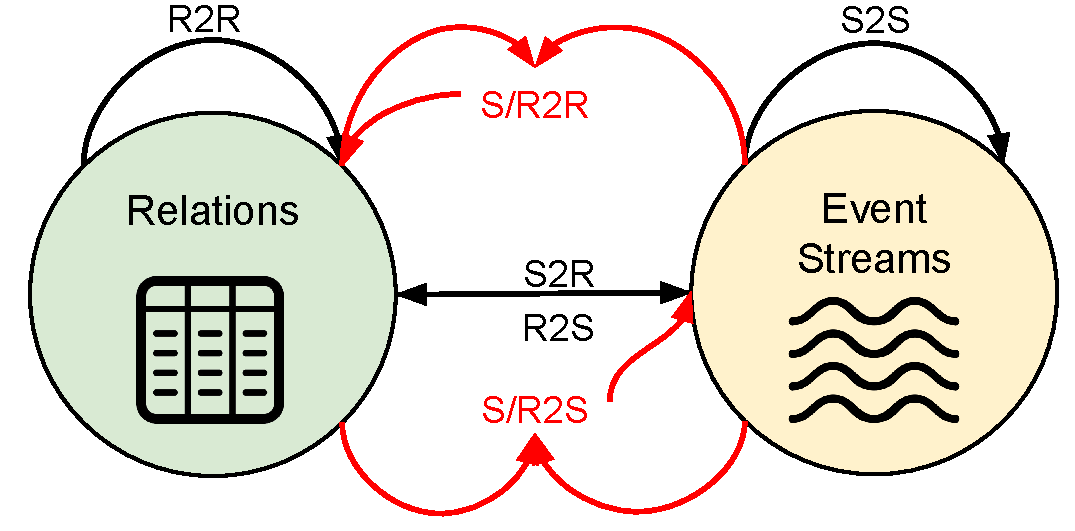
\includegraphics[width=0.55\linewidth]{StreamtoRelation.pdf}
    \caption{The CQL conceptual model: four operator families transform data between streams
    and relations~\cite{DBLP:conf/dbpl/ArasuBW03}.}
    \label{fig:CQL:model}
\end{figure}
\looseness=-1
Mixed-input families extend this base. A stream element can be enriched against a relation (a stream--relation join), with the result either updating a relation (S/R2R) or emitted onto a stream (S/R2S). Together, the S2R, R2S, S/R2R, and S/R2S families realise the \emph{stream--table duality}~\cite{sax2018streams}: stream elements upsert into an append-only relation, yielding a queryable snapshot of current state at any instant, while that relation, scanned in arrival order, replays the originating stream. This duality is the conceptual core of our approach; Section~\ref{sec:overview} instantiates it for our multi-camera tracking.

Several engines realise parts of this model. Among fully CQL-compliant systems, Stanford
STREAM~\cite{DBLP:journals/debu/ArasuBBDIMNSTVW03} pioneered the operator families but is
discontinued, while Oracle Event Processing~\cite{alves2013getting} and Apache
Flink~\cite{apacheflink} remain active; Apache Kafka Streams~\cite{DBLP:conf/edbt/JafarpourD19}
supports the same operators through a non-CQL API. Broader SQL-based streaming systems---Apache
Spark Streaming~\cite{DBLP:conf/sigmod/ArmbrustDTYZX0S18}, Samza~\cite{10.14778/3137765.3137770},
and Storm~\cite{apachestorm}---cover most families but lack full CQL syntax and, in Storm's case,
the mixed stream--relation joins central to the duality. We adopt the operator-family taxonomy
from~\cite{awad2025best} and select Esper, which
uniquely combines full CQL operator support with an embeddable, single-process JVM runtime---in
the MCOT setting additionally avoiding serialisation of high-dimensional feature tensors across
distributed workers (Section~\ref{sec:overview:realisation}). The generated EPL is portable to
other CQL-compliant engines.






\subsection{Reference Pipeline}
\label{sec:background:baseline}

As a concrete, representative instance of the monolithic architecture above, we take a state-of-the-art batch MCOT pipeline (OSC~\cite{yoshida2024overlap}), developed for
\emph{multi-camera people tracking} (MCPT), the person-specific instantiation of MCOT used throughout the AI City Challenge~\cite{wang2024aicity}; we use MCPT below only when referring to this concrete pipeline and its stages.

The pipeline comprises four stages: per-camera tracklet construction (single-camera people tracking (SCPT)), representative feature selection per track, cross-camera re-identification via similarity-based clustering, and a low-confidence detection assignment pass. Our work preserves this functional intent stage-for-stage while re-architecting it as a streams-and-tables operator graph  (Section~\ref{sec:overview}), so that tracklet state and identity mappings are maintained in queryable relational tables rather than buried in pipeline
code.



\section{Related Work}\label{sec:related}

\paragraph{Multi-Camera People Tracking: AI City Challenge Baselines}
The NVIDIA AI City Challenge~\cite{wang2024aicity} has catalysed high-performing MCPT systems. The highest-scoring 2024 offline entry, by Yoshida et al.~\cite{yoshida2024overlap}, built an \emph{Overlap Suppression Clustering} (OSC) framework that exploits future-frame context to resolve overlap anomalies (tracklets mixing multiple identities) and performs cross-camera Re-ID via pose-keypoint representative selection and average-linkage hierarchical clustering refined by world-coordinate distances. We take this exact pipeline as our functional baseline and re-architect it as a streaming program, achieving 100\% Global ID parity and $<10^{-6}$ MAD in similarity matrices \emph{online}, without offline post-processing. Other high-ranking entrants share this monolithic character while varying the association heuristics: Kim et al.~\cite{kim2024cluster} periodically re-cluster to split mixed-identity tracklets and merge duplicate global IDs; Xie et al.~\cite{xie2024robust} (the overall Track~1 winner) combine geometric consistency with state-aware Re-ID correction for camera handoffs; Specker~\cite{specker2024ocmctrack} applies a corrective matching cascade of track splitting, position-based clustering, and Re-ID rematching; and Yang et al.~\cite{yang2024online} decouple spatial clustering from world-coordinate Kalman tracking but rely on offline post-processing to correct online errors. In every case, association logic, identity state, and topology are entangled in bespoke code.

Unlike these approaches, \textbf{STREAMTRACK} employs no global per-frame bipartite matching cascades or offline correction passes. We express association as continuous SQL/EPL queries over relational state tables (\texttt{GlobalIDTable},\\ \texttt{CameraTopologyTable}), resolve identity switches and stale tracks incrementally via priority-ordered timer queries, and prune the search space from $O(N^2)$ to $O(N)$ locally via topology-aware joins---preserving functional accuracy while delivering a $9.8\times$ speedup over an equivalent JVM batch baseline.

\paragraph{Online vs.\ Offline Tracking and Scalability}
Multi-camera trackers are broadly \emph{offline}~\cite{yoshida2024overlap}, exploiting future frames for accuracy at latencies that preclude real-time use, or \emph{online}~\cite{kim2024cluster,xie2024robust,specker2024ocmctrack}, processing causally yet still relying on internal batch windows for cross-camera clustering. Critically, \emph{scalability} in this literature is treated almost exclusively as a computer-vision concern (denser crowds, more detections) rather than a \emph{systems} concern (adding cameras, reconfiguring topology, maintaining state under growth). Our work is orthogonal: we re-architect an existing offline pipeline as a streaming program, preserving its output while gaining systems-level properties---scalability via topology-aware partitioning, inspectability via queryable state, and reconfigurability via live topology updates (337\,ms outage, 190\,ms recovery, zero downtime).

\paragraph{Industrial Video Analytics Frameworks}
NVIDIA DeepStream~\cite{nvidia2024deepstream} provides GPU-accelerated single-camera tracking plugins (NvDCF, DeepSORT, IOU) but leaves cross-camera association to an external microservice layer. NVIDIA Metropolis~\cite{nvidia2025metropolis} fills this gap with a Kubernetes-based microservice architecture, but remains heavyweight and opaque: association logic is embedded in compiled services rather than declarative queries, tracking state is not directly queryable, and reconfiguration typically requires container redeployment or manual API calls rather than a single streaming event. In contrast, \textbf{STREAMTRACK} expresses association as parameterised SQL/EPL joins over a relational topology table, enabling zero-downtime reconfiguration, SQL-based state inspection, and lightweight single-process deployment.

\paragraph{Stream Processing Foundations and CEP Engine Selection}
Our approach draws on the streams-and-tables duality of Sax et al.~\cite{sax2018streams}. Distributed engines such as Apache Kafka~\cite{kreps2011kafka} and Apache Flink~\cite{carbone2015flink} offer stateful stream processing with fault tolerance, but our setting---where high-dimensional appearance tensors are shared between tracking operators and relational state---benefits from a single-process, zero-copy design. We therefore use Esper~\cite{espertech2024}, which unites SQL-like continuous queries (EPL) with first-class relational tables in an embeddable JVM runtime and supports runtime EPL (un)deployment, enabling our reactive reconfiguration loop. The closest prior CEP-for-video work, VidCEP~\cite{yadav2019vidcep}, introduced a video event query language for spatiotemporal pattern detection; as it analyses, prior event query languages~\cite{chakravarthy1994snoop,wu2006sase,cugola2010tesla,demers2007cayuga} target alphanumeric sequence matching, and database-oriented video query languages~\cite{10.1145/951676.951682,li1997moql,donderler2005bilvideo,lu2015svql,le2008query} target offline, pre-annotated repositories---neither handles continuous streaming joins. VidCEP itself targets \emph{post-tracking} event and anomaly detection over already-tracked trajectories, not the MCOT pipeline. We instead use Esper as a relational coordinator---offloading vision kernels (Re-ID, projection) to modular operators while Esper orchestrates windowing, state maintenance, and topological gating. To our knowledge, no prior work applies the streams-and-tables paradigm to the core MCOT pipeline.

\paragraph{Summary and Gap}
CV-oriented works~\cite{yoshida2024overlap,kim2024cluster,xie2024robust,specker2024ocmctrack,yang2024online} improve tracking heuristics but treat the architecture as fixed; industrial frameworks~\cite{nvidia2024deepstream,nvidia2025metropolis} offer scalable deployment without declarative logic, queryable state, or zero-downtime reconfiguration; and stream-processing~\cite{sax2018streams,carbone2015flink,kreps2011kafka} and video-CEP~\cite{yadav2019vidcep} systems provide continuous-processing foundations but have not been applied to the core MCOT pipeline. \textbf{STREAMTRACK} bridges this gap: identity is a maintained table, association a parameterised stream join, and topology a reconfigurable state relation.


\section{Architecture}\label{sec:overview}

\textbf{STREAMTRACK} instantiates the stream--table duality
(Section~\ref{sec:stream:table:duality}) for multi-camera tracking by mapping the three CQL primitives directly onto the tracking problem (Figure~\ref{fig:architecture}). \emph{Streams} carry immutable observations, per-camera detections and incremental tracklet updates. \emph{Tables} hold mutable state, the global identity mapping (\texttt{GlobalIDTable}) and the camera-network topology (\texttt{CameraTopologyTable}). \emph{Continuous queries} bridge them, consuming detection streams, reading and updating these tables, and emitting a derived \texttt{GlobalPersonEvent} stream. Casting MCOT in these terms, rather than as a bespoke imperative pipeline, is what makes the system inspectable, reconfigurable, and scalable.

% \begin{figure}[tbh!]
% \centering
% \resizebox{\linewidth}{!}{%
% \begin{tikzpicture}[
%     node distance=1.8cm and 2.5cm,
%     font=\small\sffamily,
%     streambox/.style={rectangle, draw=orange!80!black, fill=orange!8, rounded corners=3pt, minimum height=2.8em, text width=3.2cm, align=center, thick, dashed},
%     tablebox/.style={rectangle, draw=blue!70, fill=blue!8, rounded corners=3pt, minimum height=2.8em, text width=3.2cm, align=center, thick},
%     querybox/.style={rectangle, draw=black!60, fill=green!8, rounded corners=3pt, minimum height=2.8em, text width=3.2cm, align=center, thick},
%     arr/.style={-{Stealth[scale=1.1]}, thick, draw=black!60}
% ]
% \node[streambox] (s1) {\textbf{Stream}\\\scriptsize Detections, Observations};
% \node[querybox, right=of s1] (q) {\textbf{Continuous Query}\\\scriptsize EPL / SQL Operator};
% \node[streambox, right=of q] (s2) {\textbf{Derived Stream}\\\scriptsize GlobalPersonEvent};
% \node[tablebox, below=1cm of q] (t) {\textbf{State Table}\\\scriptsize GlobalIDTable, Topology};
% \draw[arr] (s1) -- node[above, font=\scriptsize] {consumes} (q);
% \draw[arr] (q) -- node[above, font=\scriptsize] {emits} (s2);
% \draw[arr, <->, draw=blue!60] (q) -- node[right, font=\scriptsize, align=left] {reads /\\updates} (t);
% \end{tikzpicture}
% }
% \caption{\textbf{STREAMTRACK}'s streams-and-tables instantiation of MCOT. Detection streams feed continuous EPL/SQL queries that maintain the \texttt{GlobalIDTable} and
% \texttt{CameraTopologyTable} as relational state and emit the derived
% \texttt{GlobalPersonEvent} stream.}
% \label{fig:duality}
% \end{figure}

The architecture is organised as a pipeline of continuous operators over detection streams and relational state tables, shown end-to-end in Figure~\ref{fig:architecture}. The same operator graph serves a single camera or an arbitrary camera network: per-camera operators (Section~\ref{sec:single}) produce local tracklet results, and cross-camera operators (Section~\ref{sec:multi}) associate them into global identities. This section specifies~\emph{what} each operator is, its inputs, outputs, processing logic, and CQL operator family, while sections~\ref{sec:single} and~\ref{sec:multi} detail \emph{how} the single- and multi-camera stages are realised.

\begin{figure*}[tbh!]
\centering
\resizebox{\textwidth}{!}{
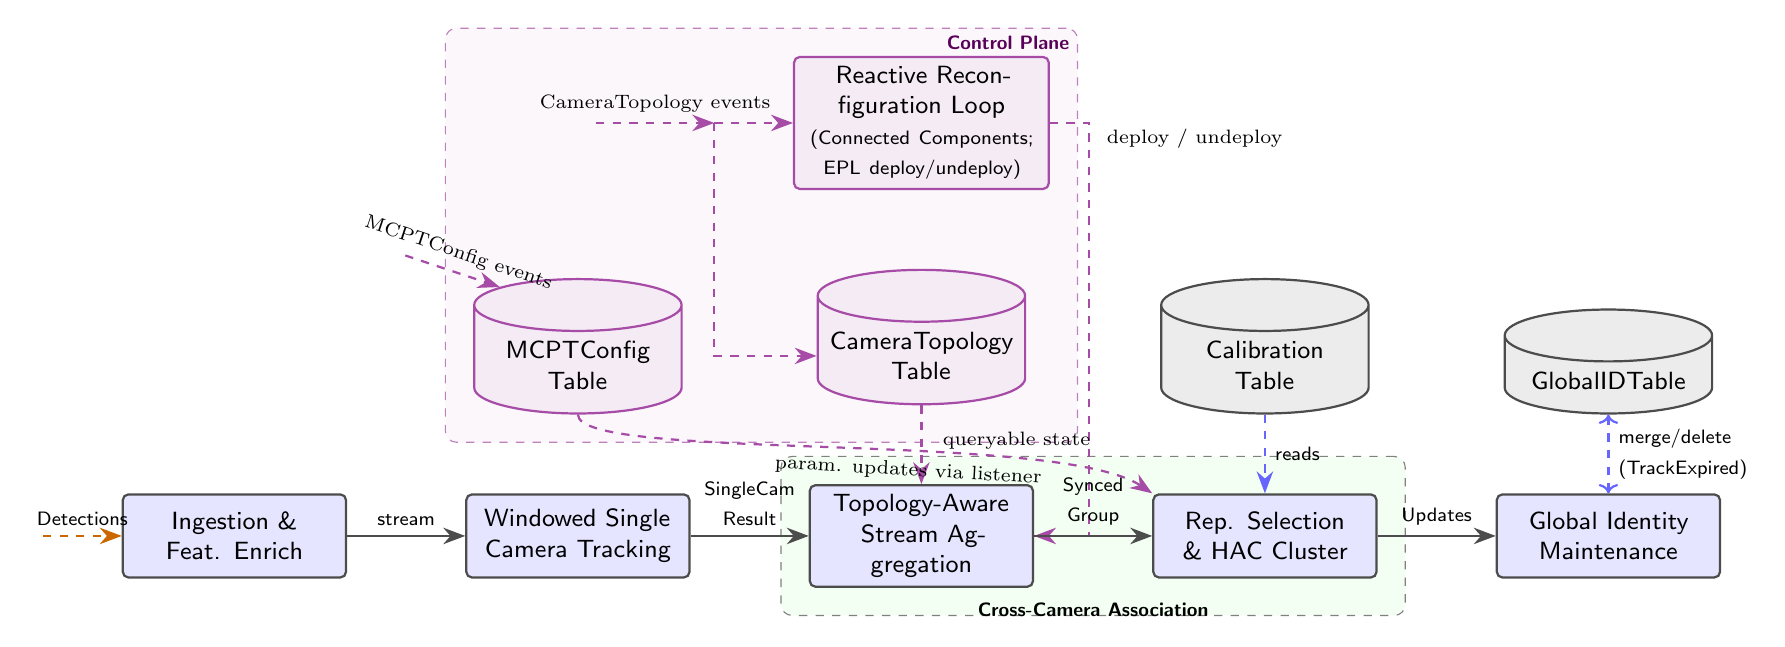
\begin{tikzpicture}[
    node distance=1.2cm and 1.5cm,
    font=\small\sffamily,
    block/.style={rectangle, draw=black!70, fill=blue!10, rounded corners=2pt, minimum height=3em, text width=2.6cm, align=center, thick},
    ctrlblock/.style={rectangle, draw=violet!70, fill=violet!8, rounded corners=2pt, minimum height=3em, text width=3.0cm, align=center, thick},
    table/.style={cylinder, shape border rotate=90, aspect=0.25, draw=black!70, fill=gray!15, text width=2.4cm, align=center, minimum height=3.5em, thick},
    ctrltable/.style={cylinder, shape border rotate=90, aspect=0.25, draw=violet!70, fill=violet!8, text width=2.4cm, align=center, minimum height=3.5em, thick},
    arrow/.style={-{Stealth[scale=1.2]}, thick, draw=black!70},
    stream/.style={-{Stealth[scale=1.2]}, thick, draw=orange!80!black, dashed},
    staterw/.style={-{Stealth[scale=1.2]}, thick, draw=blue!60, dashed},
    ctrl/.style={-{Stealth[scale=1.2]}, thick, draw=violet!70, dashed},
    group_box/.style={rectangle, draw=black!50, rounded corners=4pt, inner sep=10pt, dashed}
]
% ---------------- DATA PLANE ----------------
\node[block] (ingest) {Ingestion \& \\ Feat. Enrich};
\node[block, right=of ingest] (scpt) {Windowed Single \\ Camera Tracking};
\node[block, right=of scpt] (join) {Topology-Aware \\ Stream Aggregation};
\node[block, right=of join] (mcpt) {Rep. Selection \\ \& HAC Cluster};
\node[block, right=of mcpt] (global) {Global Identity \\ Maintenance};
\node[table, above=1.0cm of mcpt] (calibration) {Calibration\\Table};
\node[table, above=1.0cm of global] (globaltable) {GlobalIDTable};
% ---------------- CONTROL PLANE ----------------
\node[ctrltable, above=1.0cm of join] (topology) {CameraTopology\\Table};
\node[ctrltable, above=1.0cm of scpt] (configtable) {MCPTConfig\\Table};
\node[ctrlblock, above=1.0cm of topology] (reconfig) {Reactive Reconfiguration Loop\\ \scriptsize (Connected Components; EPL deploy/undeploy)};
% control event streams entering from the left
\draw[ctrl] ($ (configtable.north west) + (-1.2,0.4) $) -- node[above, font=\scriptsize, sloped] {MCPTConfig events} (configtable.north west);
% CameraTopology events: split to two parallel targets
\draw[ctrl] ($ (reconfig.west) + (-2.5,0) $) -- node[above, font=\scriptsize] {CameraTopology events} ($ (reconfig.west) + (-1.0,0) $);
\draw[ctrl] ($ (reconfig.west) + (-1.0,0) $) -- (reconfig.west);
\draw[ctrl] ($ (reconfig.west) + (-1.0,0) $) |- (topology.west);
% control wiring
\path (reconfig.east) ++(0.5,0) coordinate (rjoin);
\draw[ctrl] (reconfig.east) -- (rjoin) |- (join.east);
\path (rjoin) ++(0.1,-0.2) node[right, font=\scriptsize] {deploy / undeploy};
% table read by aggregation queries
\path (topology.south) ++(0,-0.45) coordinate (tjoin);
\draw[ctrl] (topology.south) -- (tjoin) -| (join.north);
\path (tjoin) ++(0.15,0) node[right, font=\scriptsize] {queryable state};
\draw[ctrl] (configtable.south) .. controls +(0,-0.6) and +(-1.2,0.8) .. node[below, font=\scriptsize, sloped, pos=0.6] {param. updates via listener} (mcpt.north west);
% ---------------- Data-plane arrows ----------------
\draw[stream] ($ (ingest.west) - (1cm,0) $) -- node[above] {\scriptsize Detections} (ingest.west);
\draw[arrow] (ingest) -- node[above] {\scriptsize stream} (scpt);
\draw[arrow] (scpt) -- node[above, align=center] {\scriptsize SingleCam\\ \scriptsize Result} (join);
\draw[arrow] (join) -- node[above, align=center] {\scriptsize Synced\\ \scriptsize Group} (mcpt);
\draw[arrow] (mcpt) -- node[above] {\scriptsize Updates} (global);
\draw[staterw] (calibration) -- node[right] {\scriptsize reads} (mcpt);
\draw[staterw, <->] (globaltable) -- node[right, align=left] {\scriptsize merge/delete\\ \scriptsize (TrackExpired)} (global);
% ---------------- Group backgrounds ----------------
\begin{scope}[on background layer]
    \node[group_box, fit=(join) (mcpt), fill=green!5,
      label={[anchor=base, inner sep=1pt, font=\scriptsize\bfseries\sffamily]below:Cross-Camera Association}] {};
    \node[group_box, draw=violet!50, fit=(reconfig) (configtable) (topology), fill=violet!3,
      label={[anchor=north east, inner sep=3pt, font=\scriptsize\bfseries\sffamily, text=violet!70!black]north east:Control Plane}] {};
\end{scope}
\end{tikzpicture}
}
\caption{\textbf{STREAMTRACK} operator graph with its two planes. The \emph{data plane}
(bottom) preserves the functional structure of the reference pipeline: detections arrive as
per-camera streams, single-camera tracking is a stateful windowed operator, and cross-camera
association aggregates results before global appearance clustering, with the
\texttt{CalibrationTable} and \texttt{GlobalIDTable} as relational state. The \emph{control
plane} (top, violet) carries the operational contribution: \texttt{CameraTopology} and
\texttt{MCPTConfig} events upsert into control tables (which serve as queryable state for the
operators below), and a reactive reconfiguration loop watches the \texttt{CameraTopology}
event stream, recomputes connected components, and deploys or undeploys association queries
at runtime---so both the network topology and the algorithmic parameters are reconfigurable as
data, with zero downtime.}
\label{fig:architecture}
\end{figure*}
 
% ============================================================
% Accompanying prose: INSERT immediately after the paragraph in
% Section 3 that introduces fig:architecture ("The architecture is
% organised as a pipeline of continuous operators ... realised.").
% ============================================================
 
The operator graph separates two concerns. The \emph{data plane}---ingestion, single-camera
tracking, cross-camera association, clustering, and identity maintenance---mirrors the
reference pipeline (Section~\ref{sec:background:baseline}) stage for stage; this is what makes
functional parity with the state-of-the-art baseline achievable by construction
(Section~\ref{sec:eval:parity}). The \emph{control plane} is where the architectural gains
live: \texttt{CameraTopology} and \texttt{MCPTConfig} events are themselves streams that
upsert into control tables, and a reactive reconfiguration loop watches the
\texttt{CameraTopology} event stream directly, recomputes the connected components of the
neighbourhood graph, and redeploys the affected association queries at runtime. Operational
concerns---which cameras are grouped, which thresholds apply, when queries are rebuilt---are
thus expressed in the same streams-and-tables vocabulary as the tracking itself, rather than
in configuration files or code. The data plane
answers \emph{what the baseline computes}; the control plane answers \emph{how the deployment
adapts}, and it is the latter that delivers the scalability, inspectability, and
reconfigurability properties claimed in Section~\ref{sec:background:mcot}.


\subsection{Operator Model}
\label{sec:overview:operatormodel}
Every operator in \textbf{STREAMTRACK} is specified uniformly by the streams and tables it consumes, the stream or table it produces, its processing logic, and the CQL operator
family it belongs to. Table~\ref{tab:operatormodel} gives this specification for the full pipeline; the streams and state tables it references are defined below.%\todo{student[Done]: Review the streams in/out in Table~\ref{tab:operatormodel} correct if necessary}

\begin{table*}[tbh!]
    \centering
    \caption{The \textbf{STREAMTRACK} operator model. Each operator is specified by the streams and tables it consumes, what it produces, its processing logic, and the CQL operator family it realises. Vision kernels (Re-ID embedding, homography projection, HAC) are treated as black-box UDFs invoked by the operators; the streams-and-tables layer performs the relational
    coordination.}
    \label{tab:operatormodel}
    \small
    \setlength{\tabcolsep}{4pt}
    \renewcommand{\arraystretch}{1.25}
    \begin{tabularx}{\textwidth}{@{} l X X X c @{}}
        \toprule
        \textbf{Operator} & \textbf{Input (stream / table)} & \textbf{Output} & \textbf{Processing logic} & \textbf{CQL} \\
        \midrule
        Ingestion \& Feature Enrichment
            & raw detections
            & \texttt{embeddingFeature} (stream)
            & Project and attach Re-ID embedding
            & S2S \\
        \addlinespace
        Single-Camera Tracking
            & \texttt{embeddingFeature} (stream)
            & \texttt{SingleCameraResult} (stream)
            & Windowed frame-to-frame association and post-processing (sNMS, warp, short-track exclusion)
            & S2R\,$\to$\,R2S \\
        \addlinespace
        Topology-Aware Association
            & \texttt{SingleCameraResult} (stream)
            & synced cross-camera group (stream)
            & Windowed stream aggregation parameterised by topology
            & S2R\,$\to$\,R2S \\
        \addlinespace
        Representative Selection
            & synced group (stream); \texttt{CalibrationTable}
            & \texttt{GlobalPersonEvent} (stream)
            & Keypoint/centrality selection; homography enrichment and clustering (MCPT)
            & S/R2S \\
        \addlinespace
        Global Identity Maintenance
            & \texttt{GlobalPersonEvent} (stream); \texttt{GlobalIDTable}
            & updated \texttt{GlobalIDTable}
            & Upsert (\texttt{MERGE}); materialise identity view
            & S/R2R \\
        \addlinespace
        Track Expiry \& Eviction
            & \texttt{GlobalIDTable} (timer)
            & \texttt{TrackExpiredEvent} (stream)
            & Staleness scan; emit and delete stale rows
            & R2S\,/\,R2R \\
        \bottomrule
    \end{tabularx}
\end{table*}





{\textbf{Streams and state tables.}
STREAMTRACK defines four event streams:
\schema{embeddingFeature(cameraId, curFrame, timestamp, detectedUsers[])};
\schema{SingleCameraResult(cameraId, windowIndex, clusterLabels[], featureList[], frameNumbers[], timestamps[], ...)};
\schema{GlobalPersonEvent(globalId, cameraId, serial, localId, x, y, timestamp, attributes\{\})};
and \schema{TrackExpiredEvent(globalId)}. Three state tables hold mutable state:
\schema{GlobalIDTable(globalId, lastSeen, attributes\{Cameras[], Timestamp, Coordinate\})};
\schema{CalibrationTable(cameraId, homographyMatrix)}; and
\schema{CameraTopologyTable(cameraId, neighborId, enabled, overlapping)}.\par}


Mapping~these operators onto the CQL families makes the duality concrete and shows that each MCOT challenge from Section~\ref{sec:background:mcot} is addressed by a specific operator class. Ingestion and feature enrichment are stateless stream-to-stream (S2S) mappings. Single-camera tracking pairs a stream-to-relation (S2R) window operator with a relation-to-stream (R2S) emission of \texttt{SingleCameraResult}. Cross-camera association is realised as a topology-parameterised stream aggregation (S2R\,$\to$\,R2S): the \texttt{SingleCameraResult} stream is grouped and synchronised across cameras using a windowed time-batch and a dynamic \texttt{IN(\dots)} camera-group filter, with the active query graph automatically redeployed by a reactive topology manager whenever the network topology changes. This directly addresses the \emph{scalable-association} and \emph{reconfiguration} challenges. Global identity maintenance writes each \texttt{GlobalPersonEvent} into the \texttt{GlobalIDTable} via a stream--relation merge
(S/R2R), continuously materialising the identity view, the \emph{inspectable-state} challenge, while a priority-ordered timer query emits \\\texttt{TrackExpiredEvent} (R2S) and evicts stale rows (R2R). The \texttt{GlobalIDTable} is thus both a queryable snapshot of identity and a replayable event
source: the stream--table duality in operation.

% \subsection{Execution Semantics}
% \label{sec:overview:execution}

Operators are evaluated continuously as new tuples arrive, i.e., new camera frames. Windows and joins use ingestion timestamps $\textit{ts\_ingest}$. State tables maintain current hypotheses, i.e., the assigned object ID, and apply eviction rules based on ingestion-time staleness (e.g., tracklet inactivity).



\subsection{Realisation on Esper}
\label{sec:overview:realisation}
The operator model above is engine-agnostic: any CQL-compliant engine (Section~\ref{sec:stream:table:duality}) could host it. We realise it on Esper, whose EPL language provides every operator family together with first-class relational tables, and whose embeddable single-process runtime suits the tensor-heavy MCOT setting. Sections~\ref{sec:single} and~\ref{sec:multi} give the per-operator EPL; here we state the engine-level rationale and the conventions shared across all operators.


\paragraph{Why SQL-first on a CEP engine}
Implementing MCOT via SQL/EPL on an embeddable complex-event-processing engine such as Esper~\cite{espertech2024} offers four systems-level advantages that are particularly relevant in the tensor-heavy MCOT setting:
\begin{itemize}[leftmargin=*]
    \item \textbf{Embeddable JVM-local runtime.} Esper is a lightweight library running inside the application process, enabling zero-copy sharing of appearance tensors between tracking operators and relational state in memory, without any inter-process serialisation overhead.
    \item \textbf{Relational state-table semantics.} Esper provides first-class relational tables with primary keys, indexes, and continuous transactional merges (EPL \texttt{MERGE}). This lets us model the active camera neighbourhood and global identity mappings as queryable relations that can be inspected at runtime.
    \item \textbf{Deterministic memory and tensor management.} Esper allows priority-annotated temporal queries (e.g.,\\ \texttt{TrackExpiredEvent}) that evict stale \texttt{GlobalIDTable} rows and trigger immediate JVM garbage collection of heavy vision tensors after a configurable inactivity window.
    \item \textbf{Zero-downtime topology reconfiguration.} Esper compiles, deploys, and undeploys EPL statements at runtime, so our reactive loop installs updated topological joins on-the-fly when \texttt{CameraTopology} events arrive, without interrupting tracking.
\end{itemize}
Unlike database-oriented video query systems (e.g., MOQL~\cite{li1997moql}, BilVideo~\cite{donderler2005bilvideo}, SVQL~\cite{lu2015svql}), built for static repositories, and pure pattern-matching CEP systems (e.g., Snoop~\cite{chakravarthy1994snoop}, SASE~\cite{wu2006sase}, TESLA~\cite{cugola2010tesla}), which lack mutable indexed state, Esper uniquely unites stream windowing/joins with queryable relational tables in one engine.

\paragraph{Modular operator design}
The architecture is functionally modular, akin to interchangeable ``Lego-like'' blocks. By decoupling the temporal stream-routing logic (EPL) from the heavy tracking kernels, the system permits seamless algorithm substitution. Esper handles stream synchronisation, windowing, and topological joining; when a window fills, it triggers a listener that dispatches the collected data to a native tracking operator (Figure~\ref{fig:architecture}). A developer can swap the clustering kernel (e.g., replace the default agglomerative clusterer with a density-based or deep classifier) by updating the listener registration at the engine--kernel boundary, evolving the vision logic without redesigning ingestion or synchronisation.

\paragraph{Ordering and jitter under ingestion time}
Ingestion-time semantics avoid the complexity of event-time watermarking. To absorb out-of-order delivery and jitter, the system uses a timeout-bounded aggregation window (e.g., \texttt{win:time(...) group by windowIndex having count(*) = numCameras}): the aggregation advances either when all participating cameras have reported for a \texttt{windowIndex}, or when the maximum latency expires, guaranteeing a predictable progress rate even if a camera fails to report.


\paragraph{Configuration parameters}
Runtime-tunable parameters are exposed via a \texttt{ConfigurationTable}: (i) synchronisation window size (frames), (ii) clustering similarity thresholds, (iii) neighbourhood links in the topology, and (iv) state-eviction TTLs---allowing administrators to tune the accuracy--latency trade-off dynamically.

%====================================================================
% SECTION 4: SINGLE-CAMERA OPERATORS  (Section 6 EPL absorbed per-operator)
%====================================================================
\section{Single-Camera Operators}
\label{sec:single}

These operators run independently per camera. They read only per-camera streams, touch none of the cross-camera state tables, and produce the clean \texttt{SingleCameraResult} stream that the cross-camera layer (Section~\ref{sec:multi}) consumes. This is the \emph{local} half of the two-problem decomposition introduced in Section~\ref{sec:background:mcot}. Each operator below is realised as one or more EPL statements on Esper (Section~\ref{sec:overview:realisation}).

\subsection{Ingestion and Feature Enrichment}
\label{sec:single:ingestion}

This stage ingests per-camera detections and attaches appearance-embedding vectors extracted by a pre-trained Re-ID model, emitting the \texttt{embeddingFeature} stream (a stateless S2S map). For cameras that require world locations, a continuous listener populates the \texttt{CalibrationTable} with per-camera homography matrices at ingestion time. The table is subsequently \emph{read} by the native MCPT clustering kernel (Section~\ref{sec:multi:repselect}), which projects bounding-box foot-points from the 2D image plane to a unified ground-plane coordinate system, enabling spatial gating and distance-based heuristics during cross-camera association. Thus, the \texttt{CalibrationTable} is \emph{maintained} at ingestion but \emph{consumed} downstream, consistent with its attribution to the Representative Selection row in Table~\ref{tab:operatormodel}.


Feature extraction happens at the ingestion boundary, before events enter Esper; each enriched detection is then streamed in under a per-camera event type. The per-camera event types are declared as EPL schemas once at startup:
%TODO[Student[done]]: Put proper EPL staements here.
{\small
\begin{verbatim}
-- Per-camera event schema (one per camera, 
-- derived from the Java bean)
create schema embeddingFeature_camera_0001 as
    (timestamp long, curFrame int, 
    detectedUsers java.util.List);
\end{verbatim}
}
Each camera gets its own event type name \\(\texttt{embeddingFeature\_camera\_0001}, \texttt{...0002}, etc.), which lets the downstream tracking EPL filter by stream name without adding a \texttt{cameraId} predicate to every query.

A continuous listener populates the \texttt{CalibrationTable} at ingestion time so that homography matrices are available to the downstream MCPT kernel:
{\small
\begin{verbatim}
-- Define calibration state table
create table CalibrationTable (
    cameraId int primary key,
    homographyMatrix Object);
-- Populate from incoming CameraCalibration events
insert into CalibrationTable
select cameraId, homographyMatrix 
from CameraCalibration;
\end{verbatim}
}
Once per frame, the enriched detections (Re-ID embeddings attached) are streamed to the engine under their camera-specific event type. This is the sole application-side boundary call (events originate from the detection source, i.e. camera, not from another EPL stream):
{\small
\begin{verbatim}
-- Ingestion boundary: extract features,
-- then send to Esper
EventEPLUtil.streamEvent(
    new EmbeddingFeature(timestamp, 
    frameNumber, detectedUsers),
    "embeddingFeature_camera_0001");
\end{verbatim}
}
\subsection{Single-Camera Tracking as Stateful Stream Processing}
\label{sec:single:sct}
Single-camera tracking is a stateful windowed operator\\ (S2R\,$\rightarrow$\,R2S). It maintains detection history within a sliding window (e.g., 90--120 frames) to perform frame-to-frame association, aggregating appearance features and keypoint-stability metrics per tracklet, and emits one \texttt{SingleCameraResult} event once the tracklet's window is processed. The window operator is expressed directly in EPL with a length-batch window:
{\small
\begin{verbatim}
-- Stateful windowed single-camera tracking
select detectedUsers, curFrame, timestamp
from embeddingFeature_camera_0001.win:length_batch(90)
\end{verbatim}
}
\subsection{Overlap Suppression}
\label{sec:single:overlap}

Each camera's detection stream is cleaned by an overlap-suppression step that removes redundant, overlapping bounding boxes so that each physical object yields a single best detection rather than several near-duplicate boxes. This is a standard non-maximum suppression (NMS) operation~\cite{neubeck2006efficient} %\todo{student[Done]: cite NMS / the detector's box-suppression method}
applied \emph{independently within a single camera}. In our implementation, a sequential NMS variant suppresses temporally and spatially overlapping detections at the ingestion boundary before events enter the tracking window. As a stateless S2S transformation that consumes detections and emits deduplicated ones, it precedes tracking and improves the quality of the tracklets formed downstream. By removing spurious within-camera duplicates, it also indirectly reduces false candidates entering the cross-camera join. As a detector-side post-processing step, it is applied at the ingestion boundary and has no EPL counterpart. No separate cross-camera duplicate-merge step exists; cross-camera identity resolution is handled entirely by the topology-aware association operators in Section~\ref{sec:multi}.

\paragraph{Disambiguation: overlap suppression vs.\ field-of-view overlap}

Overlap suppression must not be confused with \emph{field-of-view (FoV) overlap}, despite the shared term. Overlap suppression operates on \emph{bounding boxes within a single camera}: it is a detection-level deduplication step. FoV overlap is a \emph{multi-camera deployment property} in which two or more cameras observe the same physical region, possibly from different viewpoints. FoV overlap is a relation \emph{between} cameras, represented explicitly by the \texttt{overlapping} attribute of the \\\texttt{CameraTopologyTable} (Section~\ref{sec:multi:topology}), where it determines which cameras are grouped into synchronisation joins. The two concepts operate at different levels, pixels within a camera versus visibility across cameras, and are never combined in a single operator.


\section{Cross-Camera Operators}
\label{sec:multi}

These operators reason over two or more cameras. They consume the \texttt{SingleCameraResult} stream and read or update the cross-camera relations, \texttt{CameraTopologyTable},\\ \texttt{CalibrationTable}, and \texttt{GlobalIDTable}, to assign consistent global identities. This is the \emph{global} half of the decomposition, and where the systems-level challenges of Section~\ref{sec:background:mcot} (scalable association, inspectable state, runtime reconfiguration) are answered. As in Section~\ref{sec:single}, each operator is realised as EPL on Esper (Section~\ref{sec:overview:realisation}).

\subsection{Naive Cross-Camera Matching Cost}
\label{sec:multi:naive}
Naive cross-camera association compares tracklets across all camera pairs. For $m$ cameras, each with multiple tracklets, exhaustive matching produces a combinatorial explosion of candidate comparisons, which becomes the primary scalability bottleneck as the network grows, the \emph{scalable-association} challenge in concrete form.

\subsection{Topology-Aware Candidate Generation}
\label{sec:multi:assoc}

We formulate cross-camera association as a topology-\\parameterised stream-aggregation query synchronised by a \\\texttt{windowIndex} (an S2R\,$\to$\,R2S operator). By restricting comparisons and aggregations to localised camera groups, the candidate count drops sharply, confirmed by our 9-camera benchmark, where topology-aware partitioning yields a \textbf{4.16$\times$} reduction in per-call latency (up to \textbf{4.27$\times$} in steady state excluding JVM warm-up) relative to global matching (Section~\ref{sec:evaluation}).

Note that the query below contains \emph{no explicit join keyword}---it uses a filter predicate (\texttt{cameraId in (\dots)}) rather than a stream--table join against \texttt{CameraTopologyTable}. This is deliberate. In CQL terms the operator \emph{is} a join: it associates the detection stream with the topology relation to group cameras into synchronised clusters. The physical execution strategy, however, evaluates this join at \emph{plan time} rather than per tuple. The neighbour set is resolved once from the topology table, compiled directly into an \texttt{IN(\dots)} predicate, and baked into the deployed EPL. This is the streaming analogue of partition pruning and constant-expression folding in relational optimisers: because topology changes orders of magnitude less frequently than detections arrive, materialising the join result into the query plan eliminates a per-tuple table probe on the hot path while preserving the relational semantics. The topology relation remains the single source of truth (every deployed predicate is derivable from it), and a topology update becomes a plan change rather than a code change.
{\small
\begin{verbatim}
-- Deployed synchronised cross-camera aggregation
-- (one such query per connected component 
-- of the topology graph;
--  the IN(...) list is compiled from 
-- CameraTopologyTable at plan time)
select window( * ) as results
from SingleCameraResult(cameraId in
    ('camera_0001', 'camera_0002')).win:time(2 min)
group by windowIndex
having count(*) = 2;
\end{verbatim}
}
The aggregation query is the first half of the identity-tracking path. Once its listener dispatches grouped tracklets to the MCPT kernel, the resulting \texttt{GlobalPersonEvent}s are written into the \texttt{GlobalIDTable} via a separate on-merge statement (Section~\ref{sec:multi:globalid}), and stale entries are evicted by a priority-ordered timer query---these are the actual identity-maintenance statements.

The mechanism that populates the \texttt{IN(\dots)} predicate at plan time is the reactive reconfiguration loop described in Section~\ref{sec:multi:topology}: the \texttt{CameraTopologyTable} is maintained by an atomic upsert, and a parallel listener watches the same event stream to trigger redeployment of the affected aggregation queries with updated membership predicates.



\subsection{Camera Topology as a Reconfigurable State Table}
\label{sec:multi:topology}
A key feature is treating camera neighbourhoods as a relational configuration rather than hardcoded logic. The\\ \texttt{CameraTopologyTable} stores the active neighbour graph, where the \texttt{overlapping} flag marks pairs of cameras with \emph{shared fields of view} (Section~\ref{sec:single:overlap} contrasts this with within-camera overlap suppression). Administrators update the table at runtime by streaming \texttt{CameraTopology} events, and changes take effect for the next window of tracklets. This tables-as-data design supports zero-downtime reconfiguration (adding a camera or disabling a link) without redeploying the association queries, thereby directly addressing the \emph{runtime-reconfiguration} challenge.

The topology is declared as a relational table with a composite key, and updated at runtime by an atomic upsert driven by incoming \texttt{CameraTopology} events:
{\small
\begin{verbatim}
-- Define relational neighborhood graph
-- (Esper 9 composite primary key syntax)
create table CameraTopologyTable (
    cameraId string, neighborId string, enabled boolean, 
    overlapping boolean,
    primary key(cameraId, neighborId));

-- Update topology at runtime via atomic upsert 
on CameraTopology as ct
merge into CameraTopologyTable as target
where target.cameraId = ct.cameraId
  and target.neighborId = ct.neighborId
when matched then
  update set target.enabled = ct.enabled, 
  target.overlapping = ct.overlapping
when not matched then
  insert select ct.cameraId as cameraId,
               ct.neighborId as neighborId,
               ct.enabled as enabled,
               ct.overlapping as overlapping;
\end{verbatim}
}
Critically, the \texttt{CameraTopologyTable} is not merely a static configuration store. The system implements a \emph{reactive reconfiguration loop}: each incoming \texttt{CameraTopology} event triggers a Connected Components computation over the in-memory neighbourhood graph. When the resulting cluster partition differs from the currently active set of aggregation queries, the system automatically compiles and deploys new EPL statements targeting the updated camera groups, while undeploying the obsolete ones. This enables zero-downtime reconfiguration of the camera network; an operator can add, remove, or reassign camera neighbourhoods at runtime without restarting the pipeline or manually editing query definitions.

The reconfiguration loop itself is driven by a second EPL statement---the \emph{control-plane} counterpart to the table-upsert above. While the on-merge persists topology state, this listener detects \emph{changes} and triggers redeployment:
{\small
\begin{verbatim}
-- Reactive reconfiguration trigger: 
-- any topology change
-- redeploys the aggregation 
-- queries with updated IN(...) lists.
select * from CameraTopology;
\end{verbatim}
}
Note that this listener subscribes to the \texttt{CameraTopology} \emph{event stream}, not the table---it fires on every topology change, whereas the table upsert is a side effect. Both statements consume the same incoming event in parallel: one persists the state, the other recompiles the query plan. This is the split-entry design visible in Figure~\ref{fig:architecture} (the violet control plane). The listener's Java-side handler calls \texttt{reconcileDeployments()} which computes connected components, diffs them against the set of currently deployed aggregation queries, and for each new or changed connected component calls \texttt{deployAggregationQuery()}---the method that constructs the \texttt{IN(\dots)} clause by iterating the camera set and compiling a fresh EPL string at runtime.


\subsection{Handling Non-Overlapping Cameras via Transitional Gating}
\label{sec:multi:transition}
A challenge in real deployments is the existence of isolated (non-overlapping) cameras. If neighbourhoods are modelled purely on overlapping fields of view, a person leaving an isolated camera and entering another is assigned a new global identity, since no active stream join spans both cameras.

To resolve this without losing the benefits of topological partitioning, we introduce \emph{transition edges} in the topology graph. Unlike overlapping edges, which group cameras into synchronisation joins, transition edges define directed or bidirectional movement paths between non-overlapping regions. They are stored in the same relational \texttt{CameraTopologyTable} alongside overlapping edges, so both overlapping joins and non-overlapping transition boundaries are reconfigurable at runtime by streaming \texttt{CameraTopology} events.

For example, a person leaving the isolated view of \texttt{camera\_12} (Figure~\ref{fig:transition_flow}) may transition to \texttt{camera\_02}, \texttt{camera\_13}, or \texttt{camera\_17}. With overlapping groups alone, \texttt{camera\_12} has no neighbours and any departing track terminates, forcing a new identity on reappearance. Configuring the transitions \texttt{12:02,13,17} registers these paths.

During global association, before computing appearance similarities between active-window clusters and historical tracks in the \texttt{GlobalIDTable}, the system executes a topology-gating check:
% \begin{equation}
%     \text{Re-IDAllowed}(T_H, C_{curr}) = \begin{cases}
%         \text{True} & \text{if } \text{LastSeenCamera}(T_H) \in C_{curr} \\
%         \text{True} & \text{if } \exists c \in C_{curr} \text{ s.t. } (\text{LastSeenCamera}(T_H), c) \in E_{\text{overlap}} \cup E_{\text{transition}} \\
%         \text{False} & \text{otherwise}
%     \end{cases}
% \end{equation}

\begin{equation}
    \text{Re\text{-}IDAllowed}(T_H, C_{curr}) =
    \begin{cases}
        \text{True} & \text{if } \ell(T_H) \in C_{curr} \\
        \text{True} & \text{if } \exists\, c \in C_{curr} \text{ s.t.} \\
                    & \quad (\ell(T_H), c) \in E_{\text{ov}} \cup E_{\text{tr}} \\
        \text{False} & \text{otherwise}
    \end{cases}
\end{equation}

% where $T_H$ is the historical track, $C_{curr}$ the cameras containing the current cluster, $E_{\text{overlap}}$ the overlapping edges, and $E_{\text{transition}}$ the transition paths.
where $T_H$ is the historical track, $C_{curr}$ the cameras containing the current cluster, $\ell(\cdot)$ the last-seen camera of a track, and $E_{\text{ov}}$, $E_{\text{tr}}$ the overlapping and transition edges, respectively.

When a person leaves \texttt{camera\_12}(Figure~\ref{fig:transition_flow}), their last-seen camera in the \texttt{GlobalIDTable} is set to \texttt{camera\_12}; when a tracklet appears in \texttt{camera\_02}, \texttt{camera\_13}, or \texttt{camera\_17}, the gate admits the comparison and the global ID is preserved across the non-overlapping gap. All other cameras are bypassed, keeping the search localised and avoiding false positives in distant parts of the network.
%\todo{[done]In the figure, the dots for cameras 17 and 13 are indistinguishable}
\begin{figure*}[htb!]
    \centering
    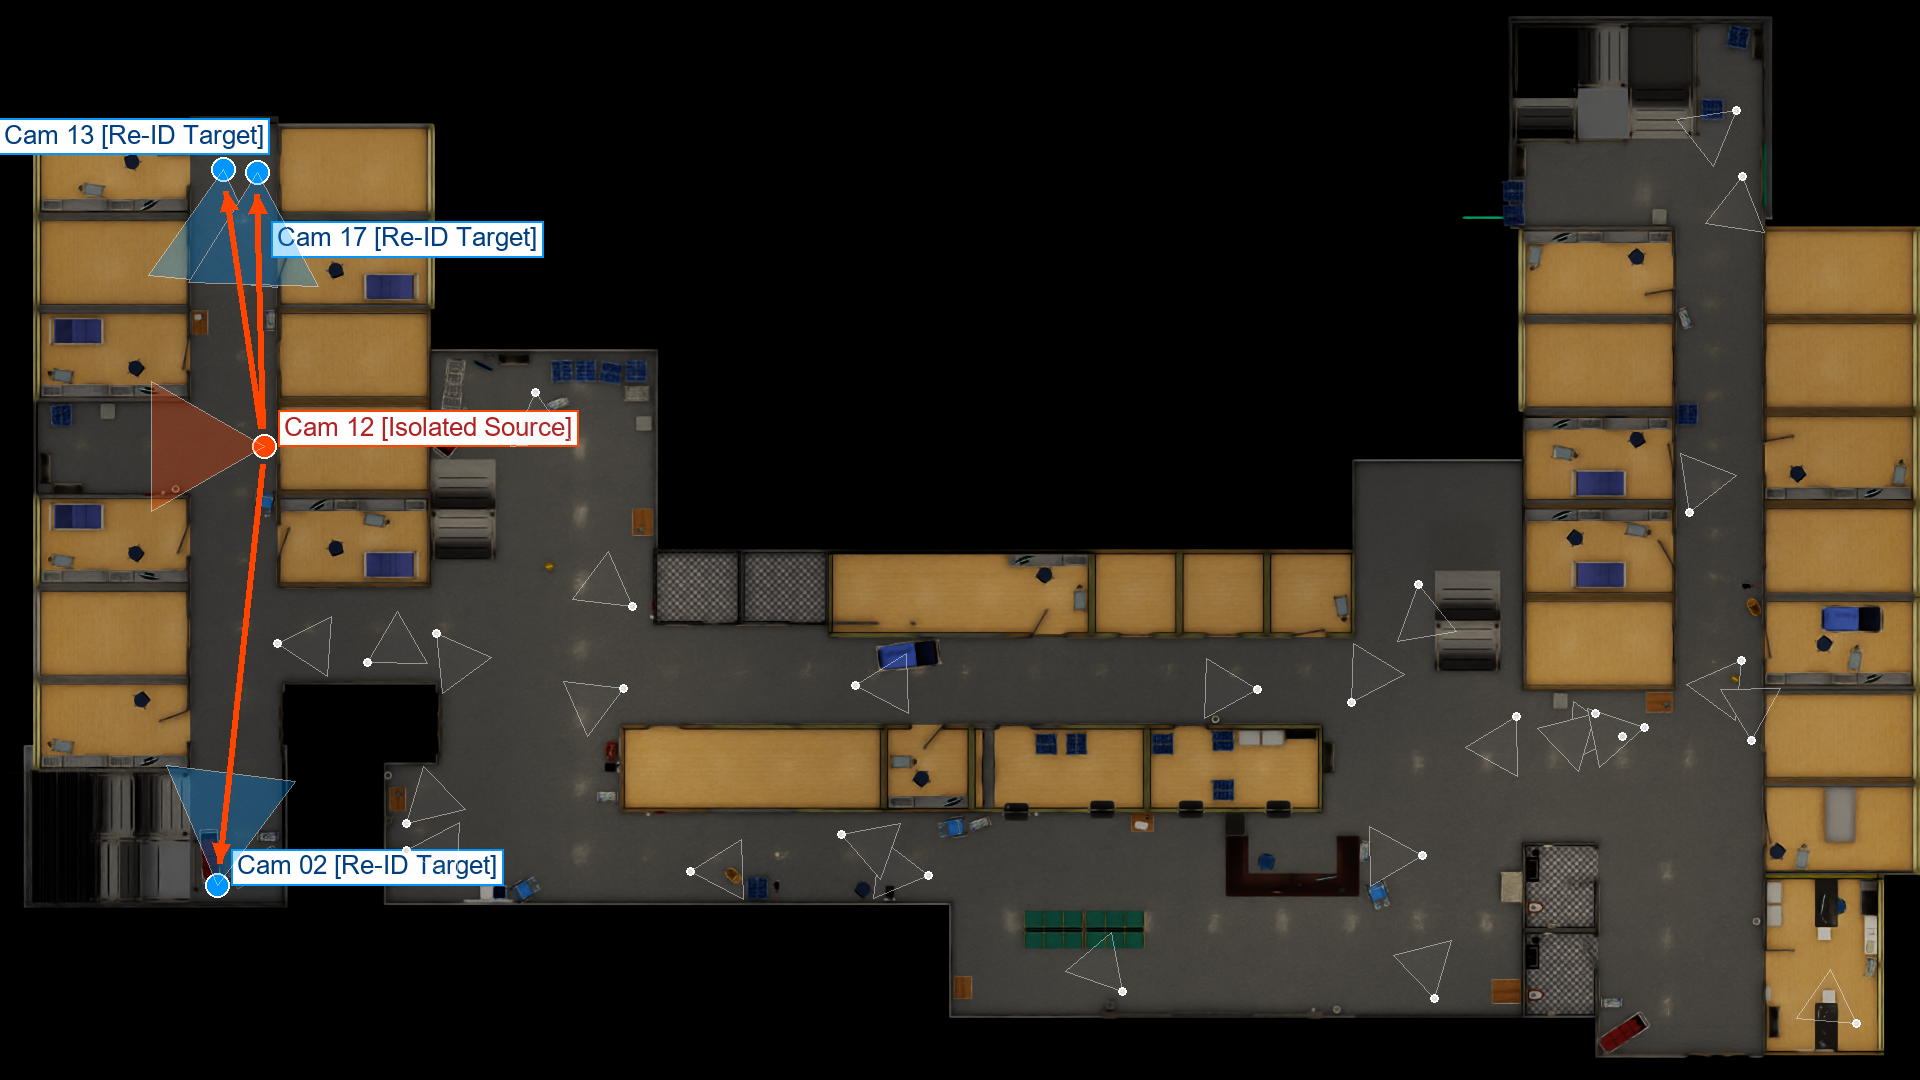
\includegraphics[width=0.65\linewidth]{./map_transition_flow.png}
    \caption{Transition topology mapping for isolated cameras. A person leaving the
    non-overlapping field of view of \texttt{Camera 12} can transition to \texttt{Camera 02},
    \texttt{Camera 13}, or \texttt{Camera 17}. Transitional gating restricts Re-ID candidate
    matching to these paths, preventing identity fragmentation across non-overlapping zones.}
    \label{fig:transition_flow}
\end{figure*}

\subsection{Representative Selection}
\label{sec:multi:repselect}

Once cameras are joined and aggregated, the MCPT module selects the top-$k$ representative observations for each associated tracklet (via an S/R2S enrichment against \texttt{CalibrationTable}). Selection uses two keypoint criteria (\texttt{keypointTh},\\ \texttt{keypointConditionTh}): (i) presence of high-confidence anatomical landmarks (facial features, limb joints), and (ii) temporal stability of appearance embeddings within the window. This ensures the subsequent Re-ID clustering operates on the most discriminative data available.

\subsection{Online Clustering and Global Identity Maintenance}
\label{sec:multi:globalid}
Global identities are maintained in the \texttt{GlobalIDTable} (an S/R2R write path). A \emph{person-centric summary} logic reduces event volume: instead of streaming per-frame coordinates, the system aggregates all sightings of a person across the synchronised cluster and emits a single \texttt{GlobalPersonEvent} per identity per window, capturing the latest sighting (\texttt{Timestamp}, \texttt{Coordinate}) and the full camera set (e.g., \texttt{Cameras:[1,2,4]}). Clustering itself is performed by a windowed Hierarchical Agglomerative Clustering (HAC) operator that executes at the end of each synchronisation window. Because the work is partitioned into topological groups, the clustering load per group remains manageable even under high-throughput streams.

The identity view is maintained by an on-merge upsert keyed by \texttt{globalId}:
{\small
\begin{verbatim}
-- Maintains GlobalIDTable with latest state 
-- and person-centric summaries
on GlobalPersonEvent as gpe
merge into GlobalIDTable as gt
where gt.globalId = gpe.globalId
when matched then
    update set gt.lastSeen = gpe.timestamp, 
    gt.attributes = gpe.attributes
when not matched then
    insert select gpe.globalId as globalId,
                  gpe.timestamp as lastSeen,
                  gpe.attributes as attributes;
\end{verbatim}
}
A key operational advantage is deterministic memory management, the \emph{inspectable-state} challenge in practice. Batch trackers often suffer from unbounded memory growth due to the accumulation of appearance signatures. Here, when the engine detects a person unseen across all cameras for a configured period (e.g., 2 minutes), a priority-ordered EPL timer emits a \texttt{TrackExpiredEvent} (R2S) and then evicts the stale rows (R2R \texttt{delete}), purging the \texttt{GlobalIDTable} and garbage-collecting the heavy feature tensors from JVM memory:
{\small
\begin{verbatim}
-- Emit TrackExpiredEvent and clean up 
-- GlobalIDTable (with Priority handling)
@Priority(10) on pattern [every timer:interval(10000)]
insert into TrackExpiredEvent 
select globalId from GlobalIDTable
where current_timestamp() - lastSeen > 120000;

@Priority(1) on pattern [every timer:interval(10000)]
delete from GlobalIDTable
where current_timestamp() - lastSeen > 120000;
\end{verbatim}
}
% TODO(consistency)[Done]: reconcile this "2 minutes" (120000 ms) expiry window with the "3-second
% synchronization window" referenced near the reconfiguration result elsewhere in the draft.
% Confirm both values.
% Confirmed: the 2-minute (120000 ms) expiry TTL and the 3-second tracking window are
% distinct parameters. The 3-second window is the per-camera SCPT tracking cycle (90 frames
% at 30 fps). The 2-minute TTL is the staleness threshold for evicting inactive global tracks
% from the GlobalIDTable.

% TODO(thin)[Done]: this subsection was originally a stub. Expanded with the candidate-reduction
% analysis (counts pruned vs. naive) below.
\subsection{Join Planning and Optimisation}
\label{sec:multi:joinplan}
Topology sparsity shrinks the join search space and improves throughput. With $m$ cameras in the global network partitioned into $k$ topology groups of sizes $n_1, \dots, n_k$ ($\sum n_i = m$), the number of pairwise candidate comparisons drops from $\binom{m}{2}$ (all-pairs) to $\sum_{i=1}^{k} \binom{n_i}{2}$, which is strictly less for $k > 1$. For our 9-camera NVIDIA SmartSpaces deployment partitioned into four groups of sizes $\{2, 2, 2, 3\}$, naive matching produces $\binom{9}{2} = 36$ camera pairs, whereas topology-aware partitioning reduces this to $1 + 1 + 1 + 3 = 6$ pairs---a $6\times$ reduction in cross-camera pair evaluations. Because each pair contributes a quadratic number of tracklet comparisons, the realised speedup at the clustering level is \textbf{4.16$\times$} (up to \textbf{4.27$\times$} in steady state excluding JVM warm-up; see Table~\ref{tab:9camera_performance}), with the residual difference attributable to varying per-group tracklet densities. Section~\ref{sec:evaluation} details the end-to-end latency measurements.


\section{Experimental Evaluation}\label{sec:evaluation}

In this section, we detail our experimental evaluation, starting with the research questions, then describing the baselines we benchmark against, the experimental setup, code porting from Python to Java, and parity checking, and finally presenting the results. The source code and instructions to reproduce the experiments will be made available in a public repository upon acceptance.


\subsection{Research Questions}
The evaluation is organised around the claim structure of the paper: the re-architecting must
first be shown to be \emph{safe} (it changes the architecture, not the answers), and only then
can its systems-level benefits---the three challenges of
Section~\ref{sec:background:mcot}---be credited to the architecture. This yields four research
questions:
 
\begin{itemize}[leftmargin=*]
    \item \textbf{RQ1 (Functional parity).} Does the streams-and-tables architecture preserve
    the tracking output of the baseline pipeline? This is the accuracy-as-invariant requirement
    of Section~\ref{sec:background:mcot}: if the answers change, no speedup is meaningful.
    Answered in Section~\ref{sec:eval:parity}.
    \item \textbf{RQ2 (Scalable association).} How much does topology-aware partitioning reduce
    candidate comparisons and per-association latency relative to global matching? This tests
    the \emph{scalable-association} claim. Answered in Section~\ref{sec:eval:topology},
    complementing the analytical reduction of Section~\ref{sec:multi:joinplan}.
    \item \textbf{RQ3 (Runtime reconfiguration).} Can the camera network be reconfigured at
    runtime without downtime or loss of tracking state? This tests the
    \emph{runtime-reconfiguration} claim, including state preservation across outage and
    recovery. Answered in Section~\ref{sec:eval:reconfig}.
    \item \textbf{RQ4 (Architectural speedup under state growth).} How does end-to-end cost
    evolve as accumulated tracking state grows over successive windows, compared to an
    equivalent batch implementation on the same runtime? This isolates the architectural
    effect---incremental processing against relational state versus per-window
    recomputation---from language and library effects. Answered in
    Sections~\ref{sec:eval:speedup} and~\ref{sec:eval:overall}.
    
\end{itemize}
 
We evaluate on the Woven VisionAI WTS dataset~\cite{kong2024wts} (functional parity and
architectural speedup, RQ1 and RQ4) and the NVIDIA SmartSpaces dataset~\cite{aicity2025track1}
(topological optimisation and runtime reconfiguration, RQ2 and RQ3), covering scenarios with
varying camera-graph sparsity and topology updates during execution. Quantitative evaluation
focuses on systems-level metrics: per-stage and end-to-end latency, cumulative cost over
successive windows, reconfiguration time, and state continuity across reconfiguration events.


\subsection{Baselines}

Baselines include: (i) a JVM-native batch-oriented pipeline that loads all features upfront and processes each window independently (\textbf{Java Batch Baseline}), (ii) the streaming streams-and-tables implementation without topology pruning (\textbf{StreamTrack-Base}), and (iii) the full optimised pipeline with topology-aware joins (\textbf{StreamTrack-Opt}). Both (i) and (ii) run on the same JVM (identical language, runtime, math library, and heap), isolating the architectural speedup from confounding language effects.

\paragraph{Baseline port and validation}
The original OSC pipeline~\cite{yoshida2024overlap} is implemented in Python. To eliminate language, runtime, and library effects from the architectural comparison, we ported it to a functionally equivalent JVM-native batch implementation (the \textbf{Java Batch Baseline} above), preserving the original stage structure, thresholds, and numerical conventions. The
port was validated against the original Python implementation on identical inputs before any streaming comparison: per-stage outputs were aligned and compared using the same parity
methodology as Section~\ref{sec:eval:parity}.

The port yields a functionally identical match. Hierarchical Agglomerative Clustering achieves perfect structural agreement (ARI = NMI = 1.0000) across all 175 commonly-aligned tracklets, and global identity cluster equivalence is 100\% (14/14 identity groups identical). The similarity matrices differ only at the level of floating-point accumulation noise: Mean Absolute Difference of $1.63 \times 10^{-8}$ for the raw cosine-similarity output, improving to $9.93 \times 10^{-9}$ after zeroing and replacement---seven orders of magnitude below any practical decision threshold ($\epsilon = 0.37$). These results confirm that the port is functionally lossless.
The evidence chain is therefore explicit: the Java batch port reproduces the published Python pipeline, and the streaming architecture reproduces the Java batch port (Section~\ref{sec:eval:parity}); by transitivity, \textbf{STREAMTRACK} preserves the functional output of the state-of-the-art baseline while every measured speedup is attributable to the architectural change alone.

\subsection{Experimental Setup}
All experiments ran on a single workstation: Windows 11 Pro (64-bit), an Intel Core i7-10610U CPU (1.80\,GHz, 4~cores / 8~threads), 32\,GB RAM, and integrated Intel UHD Graphics. The runtime was OpenJDK 21 (JBR-21.0.8, 64-Bit Server VM) with the heap fixed at 256\,MB (\texttt{-Xms256m -Xmx256m}) to emulate a resource-constrained edge environment, and the stream engine was Esper 9.0.0. Both the batch baseline and the streaming architecture were executed under these identical conditions, ensuring a fair comparison with no confounding hardware differences.




\subsection{Implementation Parity and Functional Accuracy}
\label{sec:eval:parity}
Before evaluating performance gains, we first verify that the proposed streaming architecture preserves tracking quality. Both implementations consume the identical set of pre-extracted feature embeddings per detection window, ensuring that any measured performance differences are architectural and not due to input variation. We evaluate the \emph{Implementation Parity} between the streaming streams-and-tables architecture and the JVM-native batch baseline using a serialized cross-implementation mapping method. Since the two implementations assign serial numbers in a different order (due to incremental vs. batch processing order), we align representative nodes by their unique per-tracklet serial numbers before computing all comparison metrics. Functional equivalence is quantified across five pipeline stages, spanning the full processing chain from numerical computation to final identity assignment:

\begin{itemize}[leftmargin=*]
    \item \textbf{Numerical Parity (Similarity Matrix):} We measure code-level equivalence across all three matrix stages---\texttt{RAW} (cosine similarity output), \texttt{ZEROED} (values below $\epsilon$ suppressed), and \texttt{REPLACED} (zeroed values substituted with $\delta$)---by computing the \textbf{Mean Absolute Difference (MAD)} and the fraction of cells that are bit-exact ($< 1 \times 10^{-10}$).
    \item \textbf{Structural Parity (HAC Clustering):} We compare the clustering outputs using the \textbf{Adjusted Rand Index (ARI)} and \textbf{Normalized Mutual Information (NMI)}. Both metrics are invariant to cluster-label permutation and thus capture true structural agreement.
  
   \item \textbf{Post-Processing Parity (SCPT):} We verify that the single-camera people tracking (SCPT) post-processing stages, non-maximum suppression (NMS) and warp-merge, produce identical label partitions, ensuring that all filtering and fusion heuristics are functionally equivalent.
    \item \textbf{Topology Parity (MCPT Matrix):} We confirm that the cross-camera association matrix converges to an identical structure in both pipelines.
    \item \textbf{Identity Parity (Global ID):} We confirm the final identity assigned to every physical object across the entire scene to verify absolute output consistency.
\end{itemize}

Table~\ref{tab:parity_metrics} summarizes these results for the Woven WTS Dataset.

% \begin{table*}[tbh!]
%     \centering
%     \caption{Implementation Parity: StreamTrack vs. Java Batch Baseline (Woven WTS Dataset).}
%     \label{tab:parity_metrics}
%     \begin{tabular}{@{}llc@{}}
%         \toprule
%         \textbf{Pipeline Stage} & \textbf{Metric} & \textbf{Parity Result} \\ \midrule
%         \multirow{3}{*}{Re-ID Similarity Matrix (RAW)}
%             & Mean Absolute Difference (MAD) & $1.63 \times 10^{-8}$ \\
%             & Max Difference & $1.00 \times 10^{-6}$ \\
%             & Cells Exact ($<10^{-10}$) & 98.37\% \\ \cline{2-3}
%         \multirow{2}{*}{Re-ID Similarity Matrix (ZEROED)}
%             & MAD & $0.99 \times 10^{-8}$ \\
%             & Cells Exact ($<10^{-10}$) & 99.01\% \\ \cline{2-3}
%         \multirow{2}{*}{Re-ID Similarity Matrix (REPLACED)}
%             & MAD & $0.99 \times 10^{-8}$ \\
%             & Cells Exact ($<10^{-10}$) & 99.01\% \\ \hline
%         \multirow{2}{*}{HAC Clustering}
%             & Adjusted Rand Index (ARI) & \textbf{1.0000} \\
%             & Normalized Mutual Information (NMI) & \textbf{1.0000} \\ \hline
%         \multirow{2}{*}{SCPT Post-Processing (NMS)}
%             & Adjusted Rand Index (ARI) & \textbf{1.0000} \\
%             & Unique IDs (both impl.) & 37 \\ \cline{2-3}
%         \multirow{2}{*}{SCPT Post-Processing (Warp)}
%             & Adjusted Rand Index (ARI) & \textbf{1.0000} \\
%             & Unique IDs (both impl.) & 37 \\ \hline
%         MCPT Topology Matrix & Shape Match & \textbf{12$\times$12} \\ \hline
%         Global ID Assignment & Cluster Structure Match & \textbf{100.00\%} \\ \bottomrule
%     \end{tabular}
% \end{table*}

\begin{table}[t]
    \centering
    \small
    \setlength{\tabcolsep}{4pt}
    \caption{Implementation Parity: StreamTrack vs. Java Batch Baseline (Woven WTS Dataset).}
    \label{tab:parity_metrics}
    \begin{tabular}{@{}llc@{}}
        \toprule
        \textbf{Stage} & \textbf{Metric} & \textbf{Parity} \\ \midrule
        \multicolumn{3}{@{}l}{\textit{Re-ID Similarity Matrix}} \\
        \quad RAW      & MAD & $1.63 \times 10^{-8}$ \\
                       & Max Difference & $1.00 \times 10^{-6}$ \\
                       & Cells Exact ($<10^{-10}$) & 98.37\% \\
        \quad ZEROED   & MAD & $0.99 \times 10^{-8}$ \\
                       & Cells Exact ($<10^{-10}$) & 99.01\% \\
        \quad REPLACED & MAD & $0.99 \times 10^{-8}$ \\
                       & Cells Exact ($<10^{-10}$) & 99.01\% \\ \midrule
        \multicolumn{3}{@{}l}{\textit{HAC Clustering}} \\
        \quad          & ARI & \textbf{1.0000} \\
                       & NMI & \textbf{1.0000} \\ \midrule
        \multicolumn{3}{@{}l}{\textit{SCPT Post-Processing}} \\
        \quad NMS      & ARI & \textbf{1.0000} \\
                       & Unique IDs (both impl.) & 37 \\
        \quad Warp     & ARI & \textbf{1.0000} \\
                       & Unique IDs (both impl.) & 37 \\ \midrule
        \multicolumn{3}{@{}l}{\textit{Cross-Camera}} \\
        \quad MCPT Topology Matrix & Shape Match & \textbf{12$\times$12} \\
        \quad Global ID Assignment & Cluster Match & \textbf{100.00\%} \\
        \bottomrule
    \end{tabular}
\end{table}

The metrics characterise different stages of the tracking pipeline. For the similarity matrix, MAD quantifies numerical error (where $0$ is perfect). The near-identical RAW matrices (MAD $= 1.63 \times 10^{-8}$, 98.37\% cells bit-exact) confirm that the cosine similarity computation is functionally identical between the two implementations. The small residual discrepancies ($< 1 \times 10^{-6}$) arise from floating-point accumulation differences (both implementations share the same JVM and ND4J/OpenBLAS backend) and are well below any practical decision threshold ($\epsilon = 0.37$). After zeroing and replacement, parity improves to 99.01\%.

The parity analysis was conducted incrementally during development, with each pipeline stage validated independently against the batch baseline. This process identified and resolved an identity-propagation inconsistency in the post-clustering stages, after which all stages achieve exact structural parity (ARI = NMI = 1.0000).

For clustering, the perfect ARI and NMI scores ($= 1.0000$) demonstrate that HAC produces \emph{identical} groupings---all 14 cluster groups match exactly across the 175 commonly-aligned representative nodes. The small node-selection discrepancy between the batch and streaming pipelines (the batch pipeline includes one extra representative node, serial 1018 from Camera~1) is a pre-clustering filtering artefact and does not affect the clustering outcome on the shared node set.

Beyond clustering, we verified structural parity across all downstream single-camera post-processing stages. Non-maximum suppression (NMS) produces identical labels (ARI~=~1.0000) with 37 unique identities and 893 noise-labelled detections in both implementations. The subsequent warp merge stage also achieves perfect agreement (ARI~=~1.0000, again 37 unique identities), confirming that the feature aggregation and bounding-box fusion logic are functionally equivalent. The cross-camera topology matrix, which records inter-camera association counts, converges to an identical $12 \times 12$ structure in both pipelines.

Finally, the global identity assignment achieves 100\% structural parity: all 14 global identity clusters contain the same set of (camera, serial) pairs in both implementations. The stateful \texttt{GlobalIDTable} maps incoming clusters against a persistent historical consensus of identity state, maintaining identical track associations. Consequently, all downstream tracking accuracy metrics (IDF1, HOTA) are preserved by construction, as visually affirmed in Figure~\ref{fig:visual_comparison}. 

\begin{figure*}[!t] %[tbh!]
    \centering
    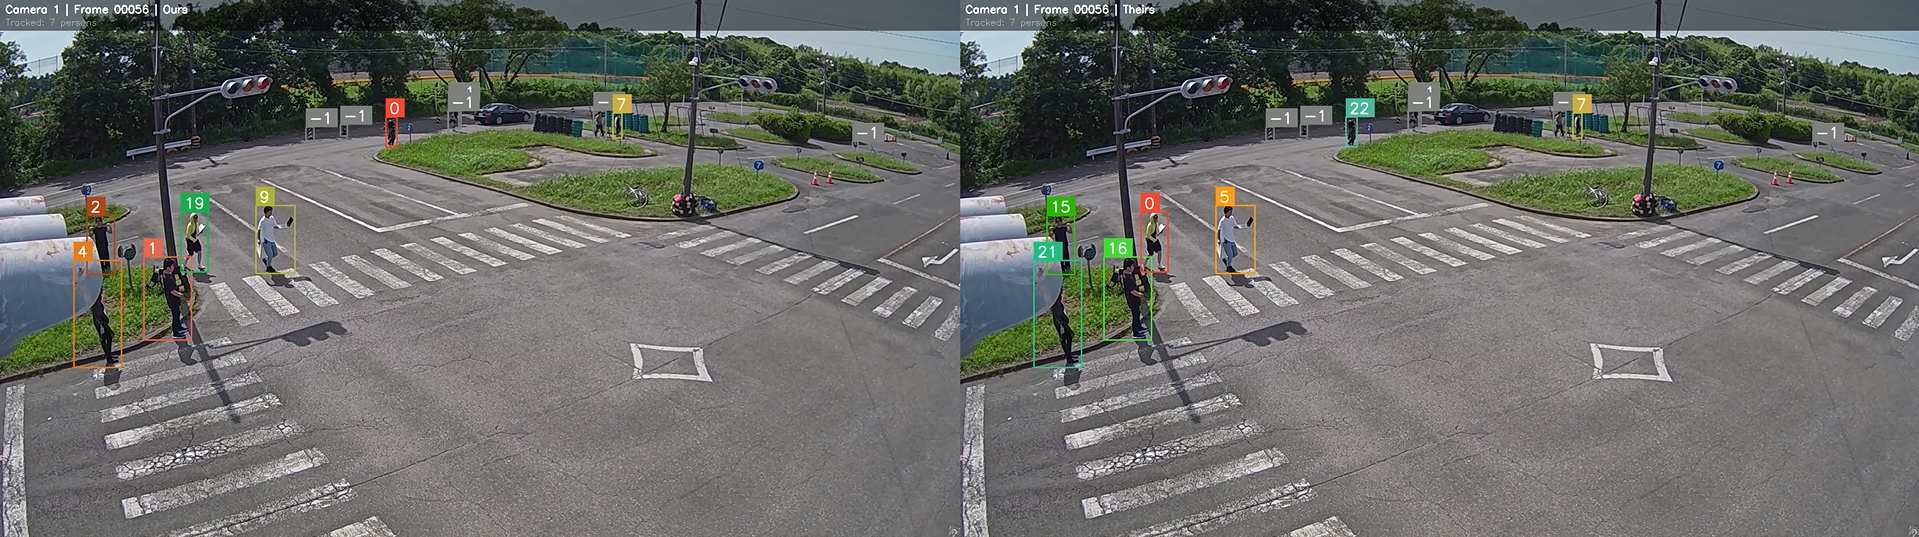
\includegraphics[width=0.8\linewidth]{./cam_01_00}
    \caption{Visual comparison of tracking results for Woven WTS Camera 01. The frame illustrates the parity between the Java batch baseline and the streaming streams-and-tables implementation, confirming that the performance optimizations do not compromise tracking coverage or identity consistency.}
    \label{fig:visual_comparison}
\end{figure*}


\subsection{Comparative Analysis of Clustering Operators}
While the streaming machine learning literature often suggests specialised algorithms such as CluStream~\cite{aggarwal2003framework} or ClusTree~\cite{kranen2011clustree} for high-velocity data, our experiments demonstrate that, for the specific window sizes encountered in MCOT (50--500 tracklets), Hierarchical Agglomerative Clustering (HAC)~\cite{mullner2011modern} is superior in both latency and identity precision. Table~\ref{tab:clustering_comparison} summarises a side-by-side benchmark conducted on the NVIDIA SmartSpaces dataset.

\begin{table}[tbh!]
    \centering
    \small
    \setlength{\tabcolsep}{4pt}
    \caption{Clustering Operator Comparison (NVIDIA SmartSpaces, 50-Window Average)}
    \label{tab:clustering_comparison}
    \begin{tabular}{@{}lrrl@{}}
        \toprule
        \textbf{Algorithm} & \textbf{Avg. Lat.} & \textbf{ID} & \textbf{Overhead} \\
                           & \textbf{(ms)}      & \textbf{Prec.} & \\ \midrule
        \textbf{HAC (Smile)} & \textbf{82.4}   & \textbf{100.0\%} & \textbf{Minimal} \\
        CluStream (MOA)      & 3{,}854.2       & 82.5\%           & High (Init) \\
        ClusTree (MOA)       & 2{,}510.8       & 78.1\%           & Moderate \\ \bottomrule
    \end{tabular}
\end{table}

The significantly higher latency of CluStream is attributed to the framework initialisation cost and the overhead of micro-clustering management, given the small $N$ per window. Furthermore, micro-clustering summaries "blur" person-specific appearance features, leading to identity merges in dense crowds where HAC maintains distinct clusters. Consequently, HAC is the only viable candidate for maintaining the functional parity reported in Table~\ref{tab:parity_metrics}.

\subsection{System Benchmark: Architectural Speedup}
\label{sec:eval:speedup}

We benchmark the performance of the proposed streams-and-tables architecture against a functionally equivalent JVM-native batch implementation of the same pipeline. Both systems are written in Java and run on the same JVM (JBR-21.0.8, heap ~256 MB) on the same workstation, isolating the architectural speedup from the confounding effects of language, runtime, and math library. The evaluation is conducted on the Woven VisionAI WTS dataset~\cite{kong2024wts} (Scene~2, cameras 0001, 0011, 0017, 0019) over 25 consecutive synchronisation windows.

Table~\ref{tab:performance_combined} summarises the architectural speedup achieved for the primary stages. Our streaming implementation significantly outperforms the batch baseline, particularly in the representative selection and hierarchical clustering stages.

\begin{table*}[tbh!]
    \centering
    \caption{Architectural Speedup (Java Batch Baseline vs. Java Streaming) for Woven WTS
    Dataset (4 cameras, Scene~2), by pipeline stage. Streaming statistics (Mean $\pm$ Std.
    Dev.) computed over 25 per-window measurements within a single cumulative run; batch
    values are from a single cumulative measurement. Stages marked with $\dagger$
    have no direct streaming equivalent.}
    \label{tab:performance_combined}
    \small
    \begin{tabular}{@{}l|rr|rr@{}}
        \toprule
        \textbf{Pipeline Stage} & \multicolumn{2}{c|}{\textbf{Batch}} & \textbf{Streaming (ms)} & \textbf{Speedup} \\
        & \textbf{ms} & \textbf{\% of total} & \textbf{Mean $\pm$ Std. Dev.} & \\ \midrule
        Clustering (HAC) & 20366.55 & 64.4\% & $86.16 \pm 68.86$ & \textbf{9.5$\times$} \\
        Representative Selection & 10235.16 & 32.4\% & $34.06 \pm 36.52$ & \textbf{12.0$\times$} \\
        Global ID Management (Assign + Reassign) & 521.00 & 1.6\% & $3.13 \pm 1.97$ & \textbf{6.7$\times$} \\
        Misc. I/O and bookkeeping & 417.19 & 1.3\% & $\dagger$ & --- \\
        Similarity Matrix Generation & 65.08 & 0.2\% & $3.67 \pm 8.28$ & --- \\
        World Coordinate Measurement & 8.65 & $<$0.1\% & $1.25 \pm 0.79$ & --- \\
        Matrix Zeroing & 6.09 & $<$0.1\% & $0.03 \pm 0.04$ & \textbf{8.6$\times$} \\
        World-Coordinate Replacement & 0.06 & $<$0.1\% & $0.002 \pm 0.010$ & $1.0\times$ \\
        \midrule
        Total Pipeline & 31620.00 & 100\% & $129.27 \pm 92.49$ & \textbf{9.8$\times$} \\
        \bottomrule
    \end{tabular}
\end{table*}


The streaming architecture's advantage is most pronounced in the two stages that dominate the total computation. \textbf{Clustering (HAC)} (batch: 20,367~ms, 64.4\% of total vs. streaming: $86.16 \pm 68.86$~ms) and \textbf{Representative Selection} (batch: 10,235~ms, 32.4\% vs. streaming: $34.06 \pm 36.52$~ms) together account for over 96\% of the batch pipeline time. The standard deviations are substantial because the first two windows incur JVM Just-In-Time (JIT) compilation overhead; excluding them, steady-state Representative Selection drops to $31.46 \pm 36.97$~ms and Clustering to $84.71 \pm 71.69$~ms. These stages are both I/O-intensive---reading pre-computed Re-ID features from disk---and compute-intensive---iterating over all pairwise tracklets in the batch case. The streaming engine exploits incremental windowing: features are pre-loaded and maintained in stateful tables, and only the new window's deltas are processed.

Of the remaining stages, only Misc.\ I/O (1.3\%) contributes measurably to the batch total, with no direct streaming equivalent. The batch Global ID Management (Assign + Reassign) is subsumed by the single Global ID Assignment stage in streaming ($3.13 \pm 1.97$~ms), delivering a \textbf{6.7$\times$} speedup. Matrix zeroing ($0.03 \pm 0.04$~ms) also benefits from incremental processing with an \textbf{8.6$\times$} speedup, while world-coordinate replacement operates at near parity ($1.0\times$). The similarity matrix generation ($3.67 \pm 8.28$~ms) and world coordinate measurement ($1.25 \pm 0.79$~ms) stages show no material speedup because their per-window streaming cost (accumulated over 25 windows) is comparable to the single-pass batch cost
(Table~\ref{tab:performance_combined}).

Overall, the streaming architecture delivers a \textbf{9.8$\times$} end-to-end speedup (cumulative over 25 windows: 3,232~ms streaming vs. 31,620~ms batch). These improvements stem from the architectural shift from batch-oriented processing---where each window incurs I/O and recomputation costs proportional to the full accumulated state---to incremental stream processing, where state lives in relational tables and per-window work is proportional only to newly arriving data.

\subsection{Topological Optimisation: NVIDIA SmartSpaces Dataset}
\label{sec:eval:topology}

While the streaming architecture provides a significant baseline improvement, the computational complexity still scales with the number of tracklets in the aggregation window. By introducing \emph{Topology-Aware Stream Joins}, we further optimise the association search space by pruning the join predicates using camera proximity. Figure~\ref{fig:topology_map} visualises this approach, showing the spatial relationship of localised tracking groups.

\begin{figure*}[tbh!]
    \centering
    
\includegraphics[width=0.85\linewidth]{./map_topology.png}
    \caption{Topological partitioning of the NVIDIA SmartSpaces network. Four topology-aware groups are shown: Group 1 (Cameras 02, 17---blue), Group 2 (Cameras 01, 11---green), Group 3 (Cameras 19, 27---orange), and Group 4 (Cameras 21, 25, 30---purple). Cameras within each group share overlapping fields of view and are joined as independent stream topologies.}
    \label{fig:topology_map}
\end{figure*}

To quantify this optimisation, we expanded the test environment to include 9 cameras (01, 02, 11, 17, 19, 21, 25, 27, 30) from the NVIDIA SmartSpaces dataset and compared the \textbf{Global} (single-group) execution against the \textbf{Topology-Aware} (4-group) partitioning. Table~\ref{tab:9camera_performance} summarises the results.



\begin{table}[tbh!]
    \centering
    \small
    \setlength{\tabcolsep}{4pt}
    \caption{Impact of Topological Optimization: Global vs. Topology-Aware (NVIDIA
    SmartSpaces). Latency in ms, Mean $\pm$ Std.\ Dev.\ over 10 independent runs.}
    \label{tab:9camera_performance}
    \begin{tabular}{@{}lccc@{}}
        \toprule
        \textbf{JIT} & \textbf{Global} & \textbf{Topology-Aware} & \textbf{Speedup} \\
        \textbf{warm-up} & \textbf{(1 grp)} & \textbf{(4 grps)} & \\ \midrule
        incl. & $41.96 \pm 22.39$ & $10.10 \pm 11.11$ & \textbf{4.16$\times$} \\
        excl. & $39.04 \pm 18.56$ & $9.15 \pm 8.27$   & \textbf{4.27$\times$} \\ \bottomrule
    \end{tabular}
\end{table}

% The results show that partitioning the NVIDIA SmartSpaces network into four topological groups reduces the average association-clustering latency by \textbf{4.16$\times$} ($41.96 \pm 22.39$ ms vs. $10.10 \pm 11.11$ ms) when including initial JVM warm-up, and by \textbf{4.27$\times$} ($39.04 \pm 18.56$ ms vs. $9.15 \pm 8.27$ ms) when excluding warm-up. These measurements are aggregated over 10 independent repetitions (runs). 

Partitioning the NVIDIA SmartSpaces network into four topological groups reduces the average association-clustering latency by \textbf{4.16$\times$} including initial JVM warm-up, and by \textbf{4.27$\times$} in steady state, aggregated over 10 independent runs (Table~\ref{tab:9camera_performance}).

Because the Java Virtual Machine (JVM) employs Just-In-Time (JIT) compilation, the first two windows of each run are significantly slower due to compilation overhead and a lack of optimisation history (the warm-up phase). Excluding these first two windows isolates the steady-state performance, where the average latency is reduced to $9.15 \pm 8.27$~ms. The standard deviation is large relative to the mean because per-window latencies are
right-skewed: most windows complete in a few milliseconds, while occasional windows with denser tracklet populations take substantially longer; the distribution is bounded below by near-zero latencies, so the dispersion reflects skew rather than instability. This
steady-state gain is primarily driven by reducing the number of tracklets processed per clustering call, localising the workload to each topological neighbourhood.


\subsection{Runtime Topology Reconfiguration}
\label{sec:eval:reconfig}

A distinctive operational advantage of \textbf{STREAMTRACK} is its ability to reconfigure the camera network topology at runtime, without any pipeline downtime, restart, or loss of tracking state. Because camera neighbourhoods are maintained as a relational \texttt{CameraTopologyTable} rather than hardcoded logic, operators can add, remove, or reassign camera links by simply injecting \texttt{CameraTopology} events into the live stream. The system's reactive reconciliation loop (\texttt{reconcileDeployments()}), triggered by a listener on the \texttt{CameraTopology} event stream, automatically recomputes the Connected Components of the updated neighbourhood graph, and atomically reconciles the deployed EPL aggregation queries. The end-to-end reconfiguration time reported in this section encompasses all three operations: (i) recomputing the Connected Components of the neighbourhood graph, (ii) undeploying EPL statements for camera groups that are no longer present in the topology, and (iii) deploying new EPL statements for the newly formed groups.

\paragraph{Key Features of Runtime Reconfiguration}
\begin{itemize}[leftmargin=*]
    \item \textbf{Zero Downtime:} The pipeline continues processing without interruption. No restart, no pause, no manual intervention.
    \item \textbf{Instant Propagation:} The new topology takes effect on the \emph{very next} synchronisation window (sub-second propagation latency).
    \item \textbf{Scoped Impact:} Only the affected camera groups are redeployed; unrelated groups remain completely untouched.
    \item \textbf{State Preservation:} The \texttt{GlobalIDTable} and all accumulated tracking state are fully preserved across the reconfiguration boundary.
\end{itemize}

We validated this capability on the NVIDIA SmartSpaces network by simulating a \textbf{camera network outage and recovery} scenario. The pipeline was initialised with the four-group topology shown in the pre-reconfiguration state of Figure~\ref{fig:reconfig_before_after} and processed two synchronisation windows (frames 1--180). At frame~180, a reconfiguration event was injected,\emph{without pausing or restarting the pipeline}, simulating a network outage that disconnects Camera~30 from its topological group (disabling links 21--30 and 25--30). This causes Camera~30 to split from the \mbox{[21, 25, 30]} cluster into a standalone group, while all other groups remain unaffected. At frame~360, a second reconfiguration event restores the links, re-merging Camera~30 back into its original group (recovery). Figure~\ref{fig:reconfig_before_after} visualises this transition on the actual floor plan.

\begin{figure*}[tbh!]
    \centering
    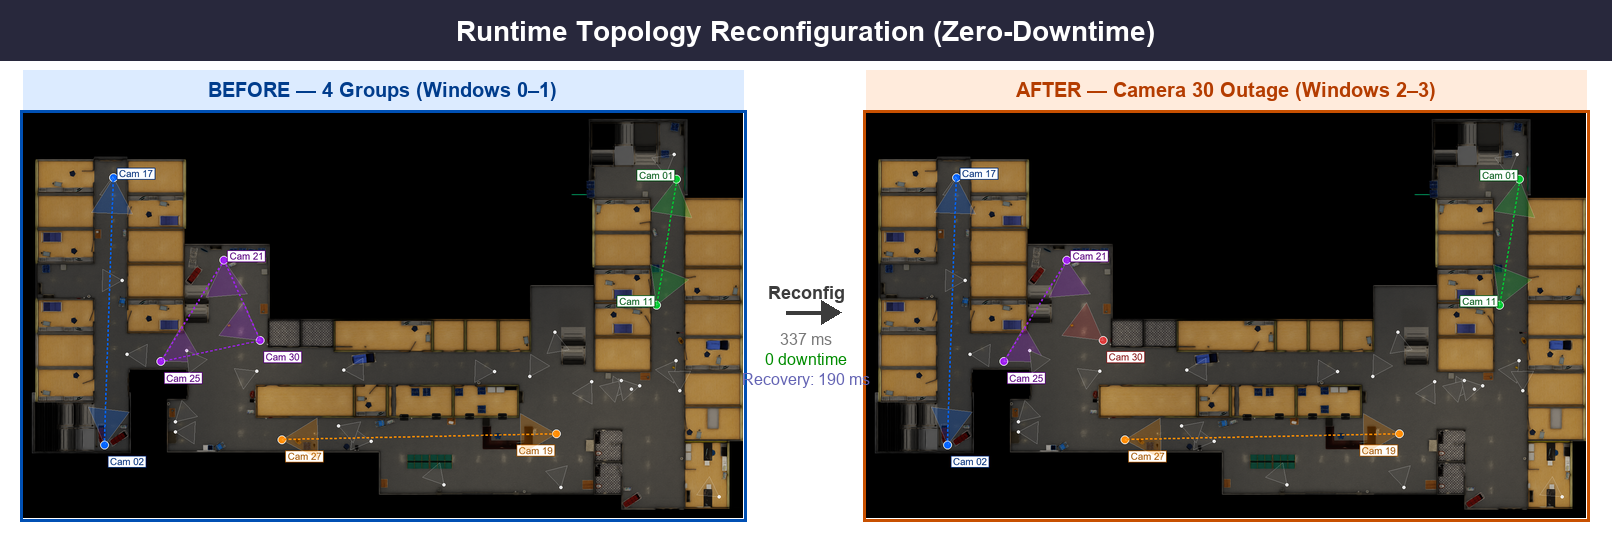
\includegraphics[width=0.9\linewidth]{./map_reconfig_combined.png}
    \caption{Runtime topology reconfiguration on the NVIDIA SmartSpaces floor plan. The left panel shows the initial four-group topology; the right panel shows the state after a Camera~30 network outage, where it is isolated as a standalone group (red). The outage transition completed in \textbf{337~ms} and the subsequent recovery in \textbf{190~ms}, both with \textbf{zero downtime}.}
    \label{fig:reconfig_before_after}
\end{figure*}

\paragraph{Results}
Table~\ref{tab:reconfiguration_timings} summarises the end-to-end reconfiguration times measured across the different types of topology changes encountered in the experiment. The initial deployment (adding all 9 individual cameras as singleton groups) takes 1759~ms, which includes JVM warm-up and initial EPL compilation overhead. The subsequent topology-aware merges, which correspond conceptually to ``add link'' operations, complete in 170--191~ms each. The outage (``disable link'') and recovery (``re-link'') transitions complete in 337~ms and 190~ms, respectively. All reconfiguration times are negligible relative to the 3-second synchronisation window.

\begin{table*}[tbh!]
    \centering
    \caption{End-to-end reconfiguration timing across topology change types. All measurements include Connected Components recomputation, EPL undeployment, and EPL deployment.}
    \label{tab:reconfiguration_timings}
    \begin{tabular}{@{}lccc@{}}
        \toprule
        \textbf{Reconfiguration Type} & \textbf{Operation} & \textbf{Deploy/Undeploy} & \textbf{Time} \\ \midrule
        Initial deployment & Add all cameras & 9 deployed, 0 undeployed & 1759~ms \\
        Topology merge ([\ldots, 0011]) & Add link & 1 deployed, 2 undeployed & 191~ms \\
        Topology merge ([\ldots, 0027]) & Add link & 1 deployed, 2 undeployed & 189~ms \\
        Topology merge ([\ldots, 0021]) & Add link & 1 deployed, 2 undeployed & 170~ms \\
        Topology merge ([\ldots, 0030]) & Add link & 1 deployed, 2 undeployed & 181~ms \\
        Camera outage (frame~180) & Disable link & 2 deployed, 1 undeployed & 337~ms \\
        Camera recovery (frame~360) & Re-link & 1 deployed, 2 undeployed & 190~ms \\ \bottomrule
    \end{tabular}
\end{table*}

\paragraph{State Preservation Evidence}
To verify that no tracking state was lost during the reconfiguration events, we inspected the \texttt{GlobalIDTable} before and after each transition. Table~\ref{tab:global_id_evidence} shows the Global IDs observed in the \texttt{camera\_0011} processing window before the outage (Window~2, frames~181--270), after the outage (Window~3, frames~271--360), and after recovery (Window~4, frames~361--450). All six Global IDs (1--6) are continuously present across all three windows, confirming that the tracking identities survived both the outage and the recovery intact. Furthermore, after the recovery re-merges Camera~30 back into \mbox{\{21, 25, 30\}}, the \texttt{camera\_0025} Global ID table adds Global ID~7 while preserving Global IDs 1--6, showing that new identities can be created normally after reconfiguration.



\begin{table}[tbh!]
    \centering
    \small
    \setlength{\tabcolsep}{4pt}
    \caption{Global IDs present in the \texttt{GlobalIDTable} before the outage (Window~2),
    after the outage (Window~3), and after recovery (Window~4). The same six Global IDs
    persist across all three windows, confirming stateful continuity.}
    \label{tab:global_id_evidence}
    \begin{tabular}{@{}llcl@{}}
        \toprule
        \textbf{Win.} & \textbf{Frames} & \textbf{Global IDs} & \textbf{Event} \\ \midrule
        2 & 181--270 & 1--6 & Before outage \\
        3 & 271--360 & 1--6 & After outage \\
        4 & 361--450 & 1--6 & After recovery \\ \bottomrule
    \end{tabular}
\end{table}


\paragraph{Beyond Topology: Runtime Parameter Reconfiguration}
The same event-driven reconfiguration pattern extends beyond topology to the behavioural parameters of the tracking algorithm itself. Just as camera neighbourhoods are maintained in the \texttt{CameraTopologyTable}, all MCPT parameters, including the similarity threshold \texttt{simTh}, the clustering radius \texttt{epsilonMcpt}, the distance metric \texttt{distanceType}, and the representative selection method, are stored in a separate \texttt{MCPTConfigTable} and can be updated at runtime by injecting \texttt{MCPTConfig} events into the live stream. A reactive listener immediately applies the change to the corresponding static field, and the next synchronisation window automatically picks up the new values because the MCPT invocation reads fresh parameter values on every call.


To demonstrate this, we inject three parameter changes at frame~270 (midway through the experiment, between the outage and recovery events): (i) tightening the similarity threshold from \texttt{simTh = 0.75} to \texttt{0.85}, (ii) reducing the clustering radius from \texttt{epsilonMcpt = 0.37} to \texttt{0.30}, and (iii) increasing the short-track pruning threshold from \texttt{shortTrackTh = 0} to \texttt{1}. All three changes are applied reactively through the same \texttt{MCPTConfigTable} infrastructure, with no pipeline restart, no code modification, and no loss of accumulated tracking state. This illustrates that the streams-and-tables architecture can serve as a general substrate for runtime-tunable multi-camera tracking, where operators can adapt both the network topology \emph{and} the algorithmic behaviour on the fly.

\subsection{Overall Performance Analysis}
\label{sec:eval:overall}

The benchmarking results across 25 consecutive data windows demonstrate that \textbf{STREAMTRACK} not only reduces single-window latency but also significantly improves total system throughput. Because both the streaming and batch implementations run on the same JVM (identical language, runtime, math library, and heap configuration), the measured speedup is purely architectural, attributable to the streams-and-tables design rather than cross-language implementation differences.

As Table~\ref{tab:performance_combined} details, the pipeline stages benefit unevenly from the streaming architecture. The \textbf{Representative Selection} exhibits the largest absolute gain (batch: 10,235~ms cumulative; streaming: $34.06 \pm 36.52$~ms per window), yielding a \textbf{12.0$\times$} speedup, because the batch pipeline re-reads and re-processes the full per-camera feature archive from disk for every window, while the streaming pipeline maintains camera state incrementally in memory. The \textbf{Clustering (HAC)} stage (\textbf{9.5$\times$}) profits similarly: batch recomputes the full hierarchical clustering over all accumulated tracklets each window, whereas streaming only clusters the new window's tracklets against the maintained identity state.

\begin{figure}[tbh!]
    \centering
    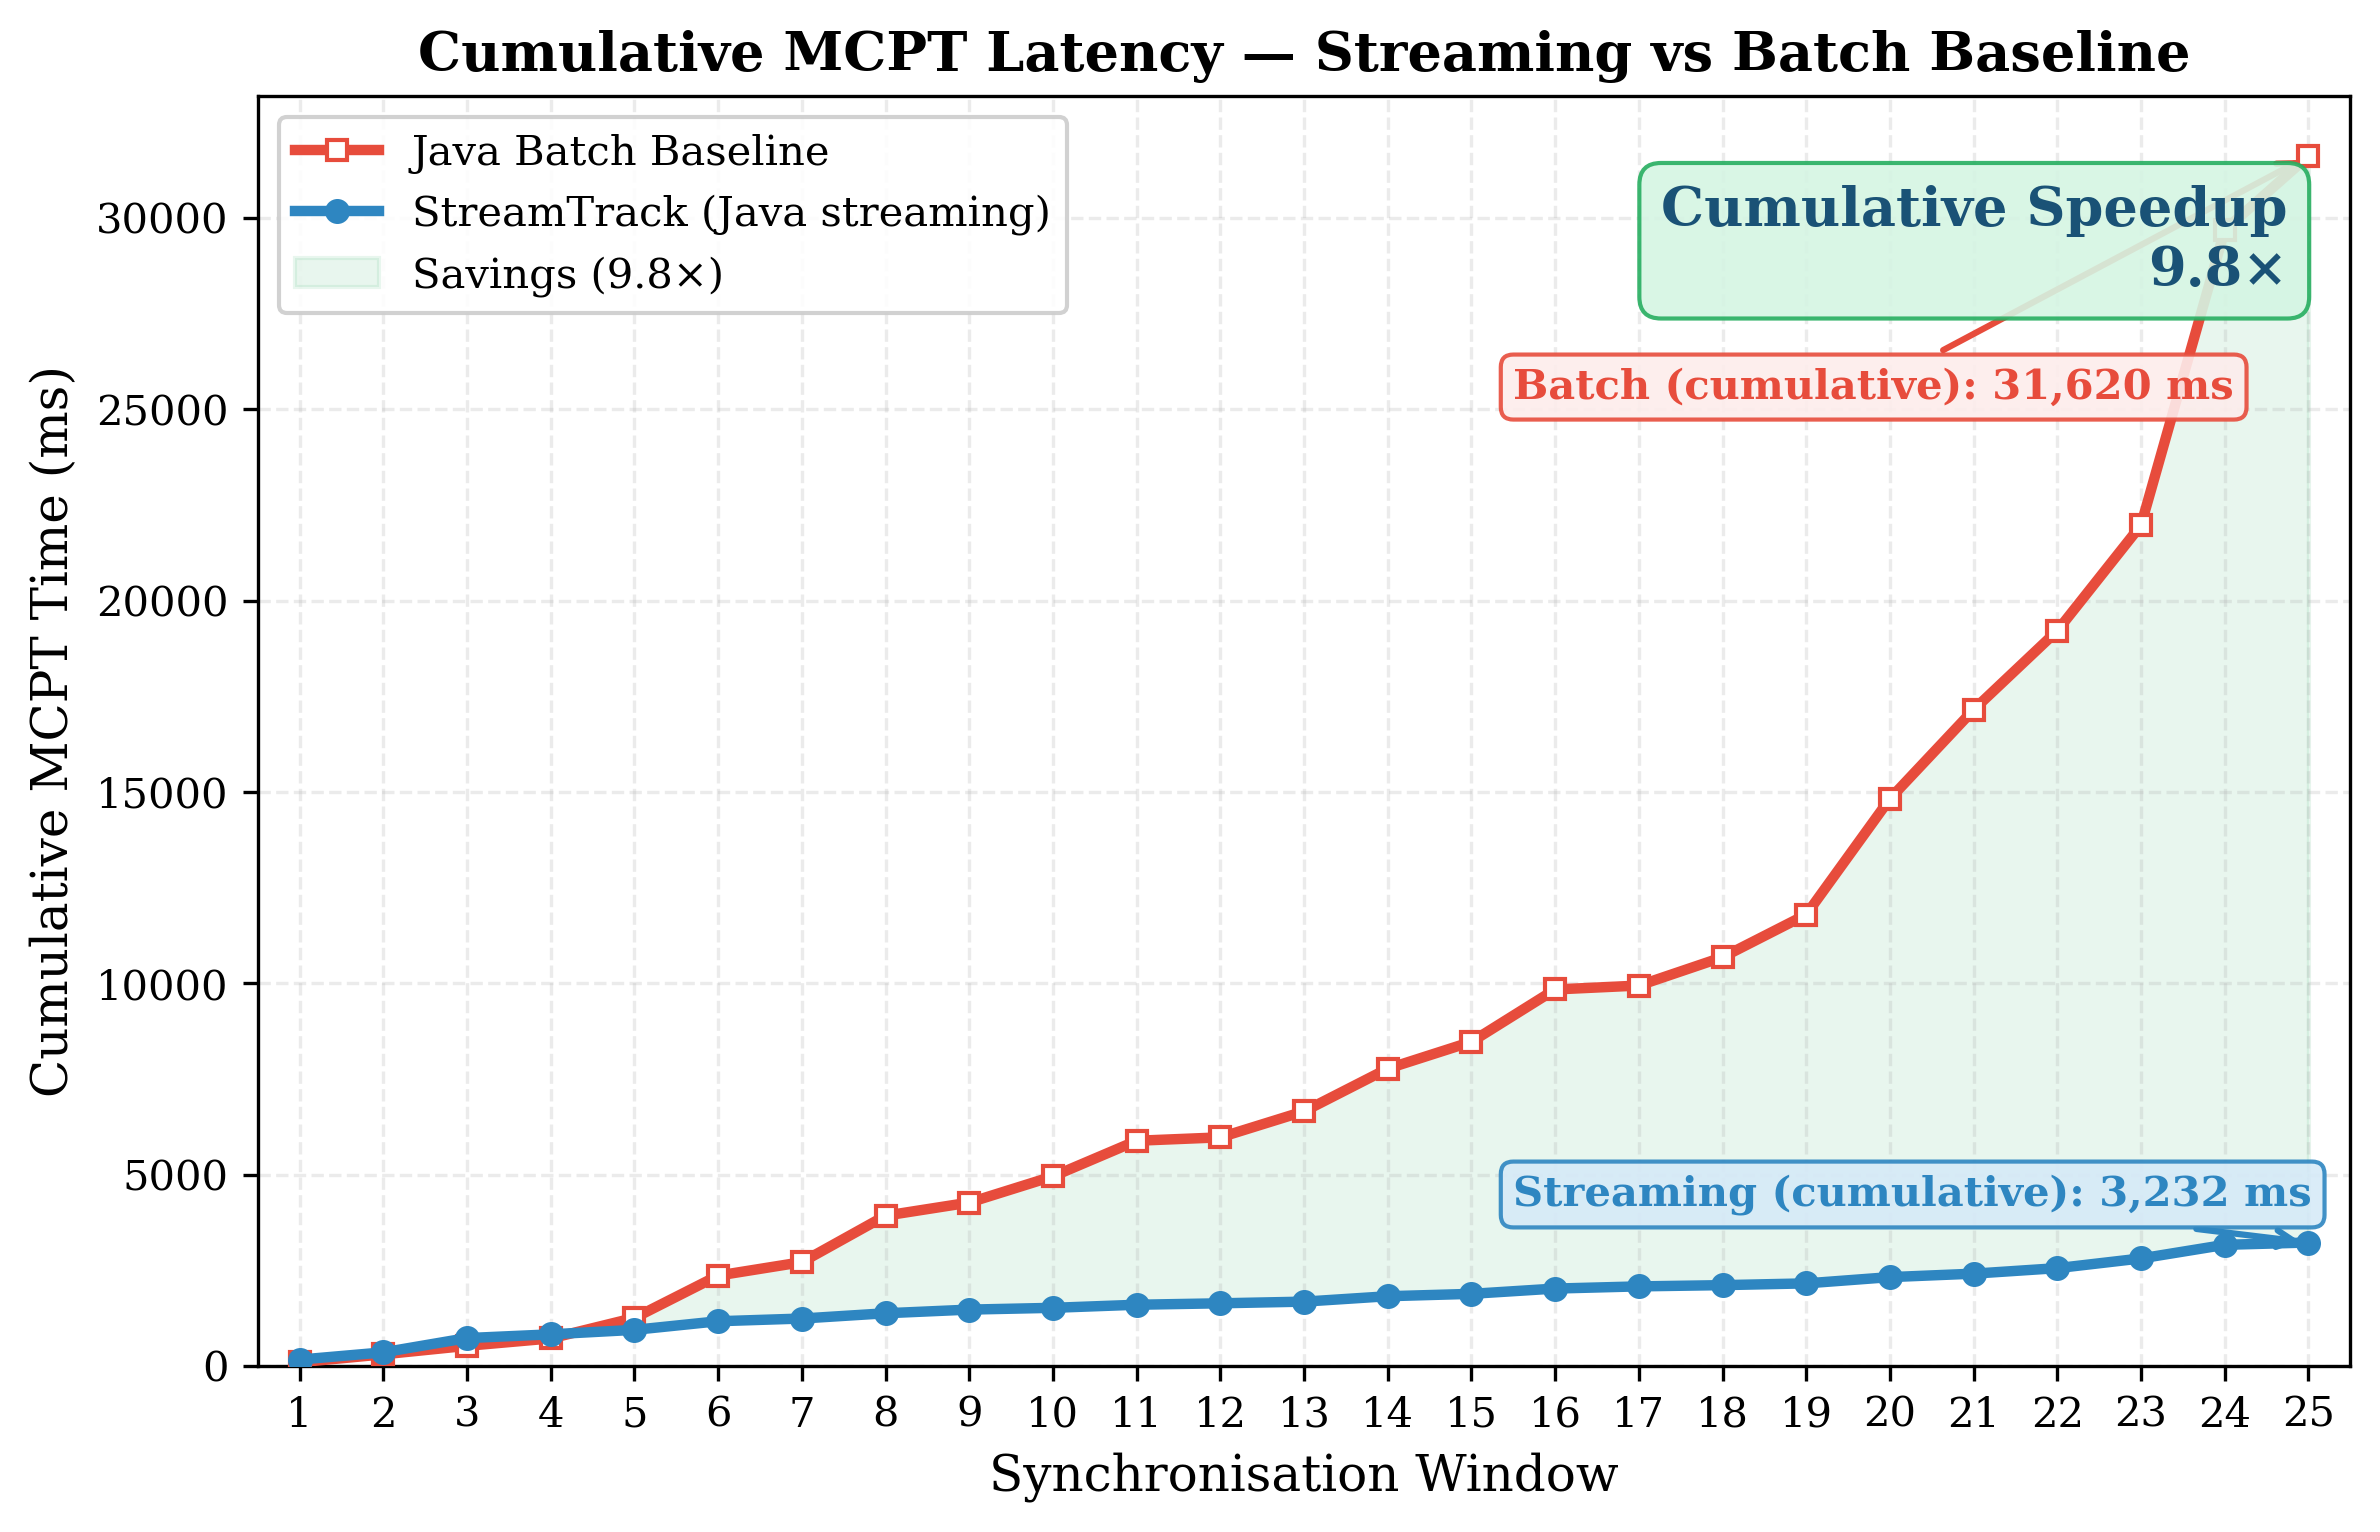
\includegraphics[width=0.9\linewidth]{./fig_cumulative_mcpt.png}
    \caption{Cumulative pipeline latency: streaming vs.\ batch baseline for the 4-camera Woven WTS dataset. The streaming pipeline processes data incrementally, accumulating to 3,232~ms over 25 windows. The batch curve is constructed from real per-window measurements: at each window $n$, the pipeline re-loads and re-processes all accumulated data from scratch, yielding a total of 31,620~ms for 25 windows. The architectural speedup reaches \textbf{9.8$\times$}.}
    \label{fig:cumulative_mcpt}
\end{figure}

Figure~\ref{fig:cumulative_mcpt} visualises the cumulative latency divergence. The streaming architecture accumulates MCPT time gradually, reaching $3,232$ ms across all $25$ windows because each window processes only newly arriving data. The batch baseline, by contrast, reprocesses the full accumulated state from scratch at every window, producing a quadratically increasing cost curve that culminates at $31,620$~ms. The cumulative speedup of \textbf{9.8$\times$} confirms that the streaming architecture neutralises the scalability bottleneck that plagues conventional batch-oriented MCPT implementations.

These results validate the central thesis of this work: the scalability limitations of MCOT are architectural rather than algorithmic. By re-architecting the pipeline around streams and tables, where state lives incrementally in relational tables and per-window processing is proportional to newly arriving data, the system sustains real-time throughput even as accumulated state grows, without sacrificing tracking fidelity. 

By defining association as a join over a reconfigurable \\\texttt{CameraTopologyTable}, the search space no longer grows with the global camera count but with the size of each topological cluster. While our largest experiment uses nine cameras, the $\binom{m}{2} \to \sum \binom{n_i}{2}$ reduction means the per-group load remains bounded as the global network grows, making deployments beyond the scale demonstrated here a plausible projection from this foundation. The bottleneck in our system has shifted from algorithmic complexity to local streaming I/O, yielding a predictable processing cost that scales with cluster size rather than the total camera count.

Because both the batch baseline and the streaming implementation share the same JVM, math library (ND4J/OpenBLAS), and heap configuration, these gains are purely architectural---they derive from the streams-and-tables design rather than from language-level performance differences. Overall, the system processes a 4-camera window in approximately 129~ms on average (streaming) vs.~1,265~ms (batch per-window average), demonstrating robust capability for real-time operation in diverse multi-camera environments.

\section{Conclusion}\label{sec:conclusion}
We presented \textbf{STREAMTRACK}, a relational streams-and-tables architecture for multi-camera object tracking. By recasting MCOT as a continuous query problem over relational state and pruning association with topology-aware stream joins, we achieved a \textbf{9.8$\times$} overall speedup over an equivalent JVM batch baseline (\textbf{12.0$\times$} in representative selection, \textbf{9.5$\times$} in clustering), with a further \textbf{4.16$\times$} (\textbf{4.27$\times$} in steady state) per-association latency reduction from topological partitioning. Because both implementations share the same language, runtime, and math library, these gains are purely architectural---validating the central claim that MCOT scalability is an architectural, not algorithmic, problem.

Beyond raw performance, the formulation yields operational benefits that monolithic pipelines lack. The system's state is \emph{inspectable}: developers can query the \texttt{GlobalIDTable} at runtime using standard SQL to audit association decisions and trace identity assignments, impossible when identity state lives in program variables. The operator graph is \emph{modular}: new vision operators (e.g., pose estimation) integrate by adding join predicates at the engine--kernel boundary, and the clustering kernel itself is swappable (Section~\ref{sec:overview:realisation}). And the deployment is \emph{reconfigurable}: both the camera topology and the algorithmic parameters are updated by streaming events, with no restart and no loss of accumulated state (Section~\ref{sec:eval:reconfig}).

The architecture also suggests a natural edge-to-cloud partitioning. The single-camera tracking stage operates independently per camera and emits compact \texttt{SingleCameraResult} events, so it can run at the edge, while the topology-aware aggregation and global clustering are centralised in the CEP engine. Our measurements support the feasibility of this split---per-window association latencies (Table~\ref{tab:9camera_performance}) sit well within edge-class budgets---and such a partitioning would reduce backhaul bandwidth from raw video to lightweight feature events while preserving a global view of identities.

Certain limitations remain. Extremely crowded scenes can produce similarity ambiguities that topological gating cannot resolve, since gating restricts \emph{where} matches are considered but not \emph{how} ambiguous appearances are disambiguated. Rapid lighting changes or occlusions can cause embedding drift, requiring online adaptation of the appearance models---an algorithmic concern deliberately outside the scope of this architectural work. Finally, our evaluation is single-node by design, to isolate architectural effects and model edge-class resource constraints; measuring the architecture across a physically distributed edge--cloud deployment is a natural next step.

Future directions include multi-hop topology reasoning, where cameras beyond immediate neighbours contribute to association via transitive similarity, and learning topology weights from historical data to dynamically adjust join selectivity.

\section*{Declaration of generative AI and AI-assisted technologies in the manuscript preparation process}
 During the preparation of this work, the authors used Claude to rephrase and shorten paragraphs. After using this tool/service, the authors reviewed and edited the content as needed and take full responsibility for the published article.
 
% \bibliographystyle{plain}
% \bibliographystyle{elsarticle-num}
% \bibliography{references}

\begin{thebibliography}{10}
\expandafter\ifx\csname url\endcsname\relax
  \def\url#1{\texttt{#1}}\fi
\expandafter\ifx\csname urlprefix\endcsname\relax\def\urlprefix{URL }\fi
\expandafter\ifx\csname href\endcsname\relax
  \def\href#1#2{#2} \def\path#1{#1}\fi

\bibitem{9151096}
Y.~Qian, L.~Yu, W.~Liu, A.~G. Hauptmann, Electricity: An efficient multi-camera vehicle tracking system for intelligent city, in: 2020 IEEE/CVF Conference on Computer Vision and Pattern Recognition Workshops (CVPRW), 2020, pp. 2511--2519.
\newblock \href {http://dx.doi.org/10.1109/CVPRW50498.2020.00302} {\path{doi:10.1109/CVPRW50498.2020.00302}}.

\bibitem{thirde2006multi}
D.~Thirde, M.~Borg, J.~Ferryman, J.~Aguilera, M.~Kampel, G.~Fernandez, Multi-camera tracking for visual surveillance applications, in: Proceedings of the Computer Vision Winter Workshop (CVWW), Czech Pattern Recognition Society, 2006.

\bibitem{bhuyan2007tracking}
M.~K. Bhuyan, B.~C. Lovell, A.~Bigdeli, Tracking with multiple cameras for video surveillance, in: 2007 International Conference on Digital Image Computing: Techniques and Applications (DICTA), 2007, pp. 592--599.
\newblock \href {http://dx.doi.org/10.1109/DICTA.2007.4426852} {\path{doi:10.1109/DICTA.2007.4426852}}.

\bibitem{yoshida2024overlap}
R.~Yoshida, J.~Okubo, J.~Fujii, M.~Amakata, T.~Yamashita, Overlap suppression clustering for offline multi-camera people tracking, in: 2024 IEEE/CVF Conference on Computer Vision and Pattern Recognition Workshops (CVPRW), Seattle, WA, USA, 2024, pp. 7153--7162.
\newblock \href {http://dx.doi.org/10.1109/CVPRW63382.2024.00710} {\path{doi:10.1109/CVPRW63382.2024.00710}}.

\bibitem{kim2024cluster}
J.~Kim, W.~Shin, H.~Park, D.~Choi, Cluster self-refinement for enhanced online multi-camera people tracking, in: 2024 IEEE/CVF Conference on Computer Vision and Pattern Recognition Workshops (CVPRW), Seattle, WA, USA, 2024, pp. 7190--7197.
\newblock \href {http://dx.doi.org/10.1109/CVPRW63382.2024.00714} {\path{doi:10.1109/CVPRW63382.2024.00714}}.

\bibitem{xie2024robust}
Z.~Xie, Z.~Ni, W.~Yang, Y.~Zhang, Y.~Chen, Y.~Zhang, X.~Ma, A robust online multi-camera people tracking system with geometric consistency and state-aware re-id correction, in: 2024 IEEE/CVF Conference on Computer Vision and Pattern Recognition Workshops (CVPRW), Seattle, WA, USA, 2024, pp. 7007--7016.
\newblock \href {http://dx.doi.org/10.1109/CVPRW63382.2024.00694} {\path{doi:10.1109/CVPRW63382.2024.00694}}.

\bibitem{sax2018streams}
M.~Sax, G.~Wang, M.~Weidlich, J.~Freytag, \href{https://doi.org/10.1145/3242153.3242155}{Streams and tables: Two sides of the same coin}, in: {BIRTE}, {ACM}, Rio de Janeiro, Brazil, 2018, pp. 1--10.
\newblock \href {http://dx.doi.org/10.1145/3242153.3242155} {\path{doi:10.1145/3242153.3242155}}.
\newline\urlprefix\url{https://doi.org/10.1145/3242153.3242155}

\bibitem{DBLP:conf/dbpl/ArasuBW03}
A.~Arasu, S.~Babu, J.~Widom, \href{https://doi.org/10.1007/978-3-540-24607-7\_1}{{CQL:} {A} language for continuous queries over streams and relations}, in: {DBPL}, Springer, Berlin, 2003, pp. 1--19.
\newblock \href {http://dx.doi.org/10.1007/978-3-540-24607-7\_1} {\path{doi:10.1007/978-3-540-24607-7\_1}}.
\newline\urlprefix\url{https://doi.org/10.1007/978-3-540-24607-7\_1}

\bibitem{awad2025best}
A.~Awad, F.~Awaysheh, H.~A. L{\'{o}}pez, \href{https://doi.org/10.1007/s44311-025-00030-8}{{BEST:} a unified business process enactment via streams and tables for service computing}, Process Sci. 2~(1).
\newblock \href {http://dx.doi.org/10.1007/S44311-025-00030-8} {\path{doi:10.1007/S44311-025-00030-8}}.
\newline\urlprefix\url{https://doi.org/10.1007/s44311-025-00030-8}

\bibitem{Bewley2016_sort}
A.~Bewley, Z.~Ge, L.~Ott, F.~Ramos, B.~Upcroft, Simple online and realtime tracking, in: 2016 IEEE International Conference on Image Processing (ICIP), 2016, pp. 3464--3468.
\newblock \href {http://dx.doi.org/10.1109/ICIP.2016.7533003} {\path{doi:10.1109/ICIP.2016.7533003}}.

\bibitem{Wojke2017_deepsort}
N.~Wojke, A.~Bewley, D.~Paulus, Simple online and realtime tracking with a deep association metric, in: 2017 IEEE International Conference on Image Processing (ICIP), 2017, pp. 3645--3649.
\newblock \href {http://dx.doi.org/10.1109/ICIP.2017.8296962} {\path{doi:10.1109/ICIP.2017.8296962}}.

\bibitem{zhang2022bytetrack}
Y.~Zhang, P.~Sun, Y.~Jiang, D.~Yu, F.~Weng, Z.~Yuan, P.~Luo, W.~Liu, X.~Wang, Bytetrack: Multi-object tracking by associating every detection box, in: Computer Vision -- ECCV 2022: 17th European Conference, Springer-Verlag, Berlin, Heidelberg, 2022, pp. 1--21.
\newblock \href {http://dx.doi.org/10.1007/978-3-031-20047-2_1} {\path{doi:10.1007/978-3-031-20047-2_1}}.

\bibitem{ye2021deep}
M.~Ye, J.~Shen, G.~Lin, T.~Xiang, L.~Shao, S.~C.~H. Hoi, Deep learning for person re-identification: A survey and outlook, IEEE Transactions on Pattern Analysis and Machine Intelligence 44~(6) (2021) 2872--2893.
\newblock \href {http://dx.doi.org/10.1109/TPAMI.2021.3054775} {\path{doi:10.1109/TPAMI.2021.3054775}}.

\bibitem{ristani2016performance}
E.~Ristani, F.~Solera, R.~Zou, R.~Cucchiara, C.~Tomasi, Performance measures and a data set for multi-target, multi-camera tracking, in: Computer Vision -- ECCV 2016 Workshops, Vol. 9914 of Lecture Notes in Computer Science, Springer, Cham, 2016, pp. 17--35.
\newblock \href {http://dx.doi.org/10.1007/978-3-319-48881-3_2} {\path{doi:10.1007/978-3-319-48881-3_2}}.

\bibitem{wang2024aicity}
S.~Wang, D.~C. Anastasiu, Z.~Tang, M.-C. Chang, Y.~Yao, L.~Zheng, M.~S. Rahman, M.~S. Arya, A.~Sharma, P.~Chakraborty, S.~Prajapati, Q.~Kong, N.~Kobori, M.~Gochoo, M.-E. Otgonbold, F.~Alnajjar, G.~Batnasan, P.-Y. Chen, J.-W. Hsieh, X.~Wu, S.~S. Pusegaonkar, Y.~Wang, S.~Biswas, R.~Chellappa, The 8th {AI} city challenge, in: 2024 IEEE/CVF Conference on Computer Vision and Pattern Recognition Workshops (CVPRW), Seattle, WA, USA, 2024.

\bibitem{nvidia2025metropolis}
{NVIDIA Corporation}, {NVIDIA Metropolis} -- multi-camera tracking {AI} workflow, \url{https://docs.nvidia.com/metropolis/}, microservices Reference Architecture 2.1. Accessed: 2026-06-18 (2025).

\bibitem{specker2024ocmctrack}
A.~Specker, {OCMCTrack}: Online multi-target multi-camera tracking with corrective matching cascade, in: 2024 IEEE/CVF Conference on Computer Vision and Pattern Recognition Workshops (CVPRW), Seattle, WA, USA, 2024, pp. 7236--7244.
\newblock \href {http://dx.doi.org/10.1109/CVPRW63382.2024.00719} {\path{doi:10.1109/CVPRW63382.2024.00719}}.

\bibitem{yang2024online}
C.-Y. Yang, H.-W. Huang, P.-K. Kim, Z.~Jiang, K.-J. Kim, C.-I. Huang, H.~Du, J.-N. Hwang, An online approach and evaluation method for tracking people across cameras in extremely long video sequence, in: 2024 IEEE/CVF Conference on Computer Vision and Pattern Recognition Workshops (CVPRW), Seattle, WA, USA, 2024, pp. 7037--7045.
\newblock \href {http://dx.doi.org/10.1109/CVPRW63382.2024.00697} {\path{doi:10.1109/CVPRW63382.2024.00697}}.

\bibitem{DBLP:journals/is/AwadTLKVS22}
A.~Awad, R.~Tommasini, S.~Langhi, M.~Kamel, E.~D. Valle, S.~Sakr, \href{https://doi.org/10.1016/j.is.2020.101679}{D\({}^{\mbox{2}}\)ia: User-defined interval analytics on distributed streams}, Inf. Syst. 104 (2022) 101679.
\newblock \href {http://dx.doi.org/10.1016/J.IS.2020.101679} {\path{doi:10.1016/J.IS.2020.101679}}.
\newline\urlprefix\url{https://doi.org/10.1016/j.is.2020.101679}

\bibitem{DBLP:journals/vldb/GiatrakosAADG20}
N.~Giatrakos, E.~Alevizos, A.~Artikis, A.~Deligiannakis, M.~N. Garofalakis, \href{https://doi.org/10.1007/s00778-019-00557-w}{Complex event recognition in the big data era: a survey}, {VLDB} J. 29~(1) (2020) 313--352.
\newblock \href {http://dx.doi.org/10.1007/S00778-019-00557-W} {\path{doi:10.1007/S00778-019-00557-W}}.
\newline\urlprefix\url{https://doi.org/10.1007/s00778-019-00557-w}

\bibitem{awaysheh2021big}
F.~M. Awaysheh, M.~Alazab, S.~Garg, D.~Niyato, C.~Verikoukis, Big data resource management \& networks: Taxonomy, survey, and future directions, IEEE Communications Surveys \& Tutorials 23~(4) (2021) 2098--2130.

\bibitem{DBLP:journals/vldb/ArasuBW06}
A.~Arasu, S.~Babu, J.~Widom, \href{https://doi.org/10.1007/s00778-004-0147-z}{The {CQL} continuous query language: semantic foundations and query execution}, {VLDB} J. 15~(2) (2006) 121--142.
\newblock \href {http://dx.doi.org/10.1007/S00778-004-0147-Z} {\path{doi:10.1007/S00778-004-0147-Z}}.
\newline\urlprefix\url{https://doi.org/10.1007/s00778-004-0147-z}

\bibitem{verwiebe2023survey}
J.~Verwiebe, P.~M. Grulich, J.~Traub, M.~Volker, Survey of window types for aggregation in stream processing systems, The VLDB Journal (2023) 1--27.

\bibitem{DBLP:conf/edbt/JafarpourD19}
H.~Jafarpour, R.~Desai, \href{https://doi.org/10.5441/002/edbt.2019.48}{{KSQL:} streaming {SQL} engine for apache kafka}, in: M.~Herschel, H.~Galhardas, B.~Reinwald, I.~Fundulaki, C.~Binnig, Z.~Kaoudi (Eds.), Advances in Database Technology - 22nd International Conference on Extending Database Technology, {EDBT} 2019, Lisbon, Portugal, March 26-29, 2019, OpenProceedings.org, Lisbon, Portugal, 2019, pp. 524--533.
\newblock \href {http://dx.doi.org/10.5441/002/EDBT.2019.48} {\path{doi:10.5441/002/EDBT.2019.48}}.
\newline\urlprefix\url{https://doi.org/10.5441/002/edbt.2019.48}

\bibitem{DBLP:conf/debs/ArtikisMUVW17}
A.~Artikis, A.~Margara, M.~Ugarte, S.~Vansummeren, M.~Weidlich, \href{https://doi.org/10.1145/3093742.3095106}{Complex event recognition languages: Tutorial}, in: Proceedings of the 11th {ACM} International Conference on Distributed and Event-based Systems, {DEBS} 2017, Barcelona, Spain, June 19-23, 2017, {ACM}, New York, NY, USA, 2017, pp. 7--10.
\newblock \href {http://dx.doi.org/10.1145/3093742.3095106} {\path{doi:10.1145/3093742.3095106}}.
\newline\urlprefix\url{https://doi.org/10.1145/3093742.3095106}

\bibitem{DBLP:journals/debu/ArasuBBDIMNSTVW03}
A.~Arasu, B.~Babcock, S.~Babu, M.~Datar, K.~Ito, R.~Motwani, I.~Nishizawa, U.~Srivastava, D.~Thomas, R.~Varma, J.~Widom, \href{http://sites.computer.org/debull/A03mar/paper.ps}{{STREAM:} the stanford stream data manager}, {IEEE} Data Eng. Bull. 26~(1) (2003) 19--26.
\newline\urlprefix\url{http://sites.computer.org/debull/A03mar/paper.ps}

\bibitem{alves2013getting}
A.~Alves, R.~J. Smith, L.~Williams, Getting Started with Oracle Event Processing 11g, Packt Publishing Birmingham, Birmingham, UK, 2013.

\bibitem{apacheflink}
{Apache Flink}, Apache flink: Stateful computations over data streams, \url{https://flink.apache.org/}, accessed: 2025-08-15 (2025).

\bibitem{DBLP:conf/sigmod/ArmbrustDTYZX0S18}
M.~Armbrust, T.~Das, J.~Torres, B.~Yavuz, S.~Zhu, R.~Xin, A.~Ghodsi, I.~Stoica, M.~Zaharia, \href{https://doi.org/10.1145/3183713.3190664}{Structured streaming: {A} declarative {API} for real-time applications in apache spark}, in: G.~Das, C.~M. Jermaine, P.~A. Bernstein (Eds.), Proceedings of the 2018 International Conference on Management of Data, {SIGMOD} Conference 2018, Houston, TX, USA, June 10-15, 2018, {ACM}, New York, NY, USA, 2018, pp. 601--613.
\newblock \href {http://dx.doi.org/10.1145/3183713.3190664} {\path{doi:10.1145/3183713.3190664}}.
\newline\urlprefix\url{https://doi.org/10.1145/3183713.3190664}

\bibitem{10.14778/3137765.3137770}
S.~A. Noghabi, K.~Paramasivam, Y.~Pan, N.~Ramesh, J.~Bringhurst, I.~Gupta, R.~H. Campbell, \href{https://doi.org/10.14778/3137765.3137770}{Samza: stateful scalable stream processing at linkedin}, Proc. VLDB Endow. 10~(12) (2017) 1634–1645.
\newblock \href {http://dx.doi.org/10.14778/3137765.3137770} {\path{doi:10.14778/3137765.3137770}}.
\newline\urlprefix\url{https://doi.org/10.14778/3137765.3137770}

\bibitem{apachestorm}
{Apache Storm}, Apache storm, \url{https://storm.apache.org/}, accessed: 2025-08-15 (2025).

\bibitem{nvidia2024deepstream}
{NVIDIA Corporation}, {NVIDIA DeepStream SDK} -- streaming analytics toolkit for {AI}-based multi-sensor processing, \url{https://developer.nvidia.com/deepstream-sdk}, version 7.x. Accessed: 2026-06-18 (2024).

\bibitem{kreps2011kafka}
J.~Kreps, N.~Narkhede, J.~Rao, {Kafka}: A distributed messaging system for log processing, in: Proceedings of the Workshop on Networking Meets Databases (NetDB), 2011.

\bibitem{carbone2015flink}
P.~Carbone, A.~Katsifodimos, S.~Ewen, V.~Markl, S.~Haridi, K.~Tzoumas, Apache {Flink}: Stream and batch processing in a single engine, IEEE Data Engineering Bulletin 38~(4) (2015) 28--38.

\bibitem{espertech2024}
E.~Inc., Esper -- complex event processing engine, \url{https://www.espertech.com/esper/}, version 9.x. Accessed: 2026-03-13 (2024).

\bibitem{yadav2019vidcep}
P.~Yadav, E.~Curry, {VidCEP}: Complex event processing framework to detect spatiotemporal patterns in video streams, in: 2019 IEEE International Conference on Big Data (Big Data), 2019, pp. 2513--2522.
\newblock \href {http://dx.doi.org/10.1109/BigData47090.2019.9006018} {\path{doi:10.1109/BigData47090.2019.9006018}}.

\bibitem{chakravarthy1994snoop}
S.~Chakravarthy, D.~Mishra, Snoop: An expressive event specification language for active databases, Data \& Knowledge Engineering 13~(3) (1994) 301--326.

\bibitem{wu2006sase}
E.~Wu, Y.~Diao, S.~Rizvi, High-performance complex event processing over streams, in: Proceedings of the 2006 ACM SIGMOD international conference on Management of data (SIGMOD), 2006, pp. 407--418.

\bibitem{cugola2010tesla}
G.~Cugola, A.~Margara, {TESLA}: a formally defined event specification language, in: Proceedings of the Fourth ACM International Conference on Distributed Event-Based Systems (DEBS), 2010, pp. 50--61.

\bibitem{demers2007cayuga}
A.~Demers, J.~Gehrke, B.~Panda, M.~Riedewald, V.~Sharma, W.~White, Cayuga: A general purpose event monitoring system, in: Proceedings of the Third Biennial Conference on Innovative Data Systems Research (CIDR), 2007, pp. 412--422.

\bibitem{10.1145/951676.951682}
W.~Aref, M.~Hammad, A.~C. Catlin, I.~Ilyas, T.~Ghanem, A.~Elmagarmid, M.~Marzouk, \href{https://doi.org/10.1145/951676.951682}{Video query processing in the vdbms testbed for video database research}, in: Proceedings of the 1st ACM International Workshop on Multimedia Databases, MMDB '03, Association for Computing Machinery, New York, NY, USA, 2003, p. 25–32.
\newblock \href {http://dx.doi.org/10.1145/951676.951682} {\path{doi:10.1145/951676.951682}}.
\newline\urlprefix\url{https://doi.org/10.1145/951676.951682}

\bibitem{li1997moql}
J.~Z. Li, M.~T. Ozsu, D.~Szafron, V.~Oria, {MOQL}: A multimedia object query language, in: Proceedings of the 3rd International Workshop on Multimedia Information Systems, 1997, pp. 115--124.

\bibitem{donderler2005bilvideo}
M.~E. Donderler, E.~Saykol, U.~Arslan, O.~Ulusoy, U.~Gudukbay, {BilVideo}: Design and implementation of a video database management system, Multimedia Tools and Applications 27~(1) (2005) 79--104.

\bibitem{lu2015svql}
C.~Lu, M.~Liu, Z.~Wu, {SVQL}: A {SQL} extended query language for video databases, International Journal of Database Theory and Application 8~(4) (2015) 109--118.

\bibitem{le2008query}
T.~L. Le, M.~Thonnat, A.~Boucher, F.~Bremond, A query language combining object features and semantic events for surveillance video retrieval, in: Proceedings of the 14th International Conference on Multimedia Modeling (MMM), 2008, pp. 209--220.

\bibitem{neubeck2006efficient}
A.~Neubeck, L.~Van~Gool, Efficient non-maximum suppression, in: 18th International Conference on Pattern Recognition (ICPR'06), Vol.~3, IEEE, 2006, pp. 850--855.
\newblock \href {http://dx.doi.org/10.1109/ICPR.2006.479} {\path{doi:10.1109/ICPR.2006.479}}.

\bibitem{kong2024wts}
Q.~Kong, Y.~Kawana, R.~Saini, A.~Kumar, J.~Pan, T.~Gu, Y.~Ozao, B.~Opra, D.~C. Anastasiu, Y.~Sato, N.~Kobori, \href{https://arxiv.org/abs/2407.15350}{Wts: A pedestrian-centric traffic video dataset for fine-grained spatial-temporal understanding}, homepage: \url{https://woven-visionai.github.io/wts-dataset-homepage/} (2024).
\newblock \href {http://arxiv.org/abs/2407.15350} {\path{arXiv:2407.15350}}.
\newline\urlprefix\url{https://arxiv.org/abs/2407.15350}

\bibitem{aicity2025track1}
NVIDIA, A.~Challenge, Ai city challenge 2025 track 1: Multi-camera people tracking, \url{https://www.aicitychallenge.org/2025-track1/}, data hosted at \url{https://huggingface.co/datasets/nvidia/PhysicalAI-SmartSpaces}. Accessed: 2026-03-13 (2025).

\bibitem{aggarwal2003framework}
C.~C. Aggarwal, J.~Han, J.~Wang, P.~S. Yu, A framework for clustering evolving data streams, in: Proceedings of the 29th International Conference on Very Large Data Bases (VLDB), VLDB '03, VLDB Endowment, 2003, pp. 81--92.

\bibitem{kranen2011clustree}
P.~Kranen, I.~Assent, C.~Baldauf, T.~Seidl, The {ClusTree}: Indexing micro-clusters for anytime stream mining, Knowledge and Information Systems 29~(2) (2011) 249--272.
\newblock \href {http://dx.doi.org/10.1007/s10115-010-0342-8} {\path{doi:10.1007/s10115-010-0342-8}}.

\bibitem{mullner2011modern}
D.~M{\"u}llner, Modern hierarchical, agglomerative clustering algorithms, arXiv preprint arXiv:1109.2378.

\end{thebibliography}


\end{document}
